\chapter{Structure-Based Virtual Screening}

Tenofovir disoproxil fumarate (TDF) (Figure \ref{fig:Viread}), a drug approved by US Food and Drug Administration (FDA) for the treatments of both human immunodeficiency virus (HIV) in 2001 and hepatitis B virus (HBV) in 2008, has recently been proved to be more effective and less expensive than another drug adefovir dipivoxil in inhibiting the reverse transcriptases (RTs). However, TDF exhibits toxicity towards S-Adenosyl-L-Homocysteine hydrolase (SAHH), adenosine deaminase (ADA), and purine nucleoside phosphorylase (PNP), three essential enzymes that are needed by human body.

\begin{figure}
\centering
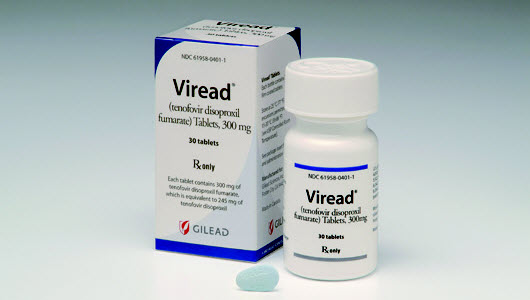
\includegraphics[width=\textwidth]{VirtualScreening/Figures/Viread.jpg}
\caption{Tenofovir disoproxil fumarate (Tradename: Viread).}
\label{fig:Viread}
\end{figure}

\section{Problem Definition}

The problem is to discover a new drug that inhibits HIV RT only, without affecting SAHH, ADA, or PNP. From the computational perspective, it is equivalent to shortlisting candidates from existing ligand databases such that they bind to HIV RT with a higher affinity and bind to SAHH, ADA, and PNP with a lower affinity.

\section{Motivation}

Shortlisting promising ligands against certain proteins can be done by virtual screening. AutoDock Vina \citep{595-2010} is a competitive tool well known for its fast execution and high accuracy. Nevertheless, it does not natively support virtual screening. When docking a massive number of ligands, it is fast, but just not fast enough. There are tremendous requests for modifying Vina, making it support virtual screening in a superfast manner.

\section{Medicinal Background}

According to the fact sheets of World Health Organization, since the beginning of AIDS epidemic, almost 60 million people have been infected with HIV and 25 million people have died of HIV-related causes. At the end of 2010, more than 34 million people were living with HIV, up from 26.2 million people in 1999. Sub-Saharan Africa is the most affected region and is home to 67\% of all people living with HIV worldwide and 89\% of all new infections among children. Asia is the second-worst affected region with 4.9 million people living with HIV. Among them, 4.1 million were in South and South-East Asia, and 0.77 million were in East Asia (Figure \ref{HIVPopulationDistribution}, reprinted from the 2010 edition of the UNAIDS Report on the global AIDS epidemic.). In 2009 alone, 2.6 millions people were newly infected, down from a peak of 3.2 million in 1997, and 1.8 million people died of AIDS, down from a peak of 2.1 million in 2004.

\begin{figure}
\centering
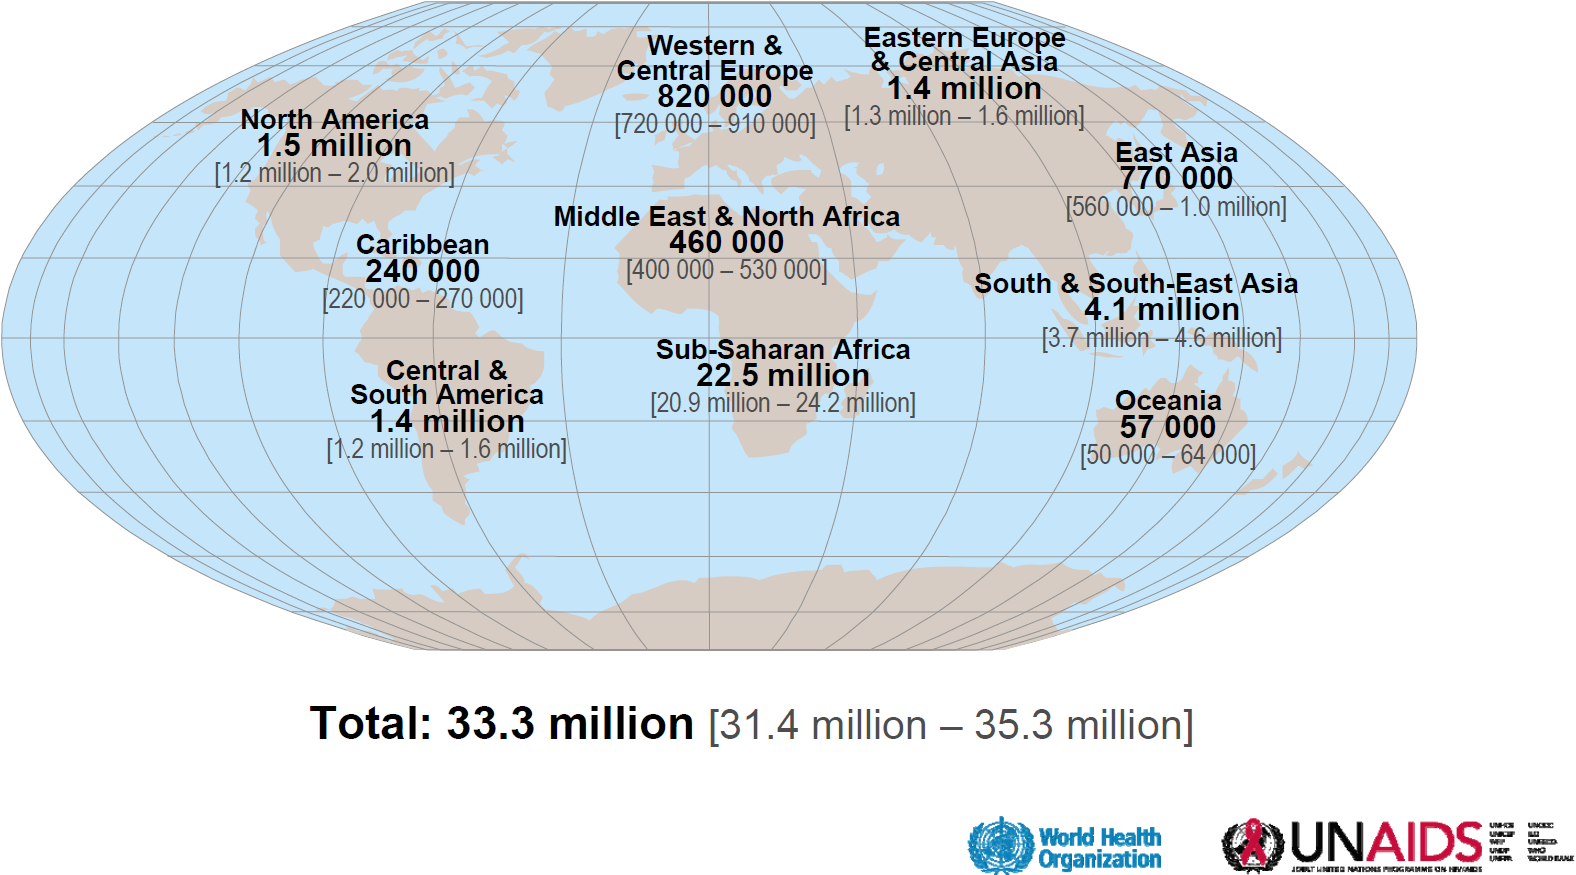
\includegraphics[width=\textwidth]{VirtualScreening/Figures/HIVPopulationDistribution.png}
\caption{Adults and children estimated to be living with HIV at the end of 2009. Figure reprinted from the 2010 edition of the UNAIDS Report on the global AIDS epidemic.}
\label{HIVPopulationDistribution}
\end{figure}

Human immunodeficiency virus (HIV) (Figure \ref{subfig:HIVDiagram}, reprinted from US National Institute of Health) is a retrovirus that causes acquired immune deficiency syndrome (AIDS), a condition in humans in which progressive failure of the immune system allows life-threatening opportunistic infections and cancers to thrive. Figure \ref{subfig:HIVReplicationCycle} \citep{296-2010} shows the replication cycle of HIV. Upon entry into the target cell, the single-stranded viral RNA genome is reverse transcribed into double-stranded DNA by a viral reverse transcriptase (HIV RT) that is transported along with the viral genome in the virus particle. The resulting viral DNA is then imported into the cell nucleus and integrated into the cellular DNA by a viral integrase. Once integrated, the virus may become latent, allowing the virus and its host cell to avoid detection by the immune system. Alternatively, the virus may be transcribed by a viral protease (HIV PR), producing new RNA genomes and viral proteins that are packaged and released from the cell as new virus particles that begin a new replication cycle.

\begin{figure}
\centering
\subfigure[Diagram of HIV. Figure reprinted from US National Institute of Health.]
{
  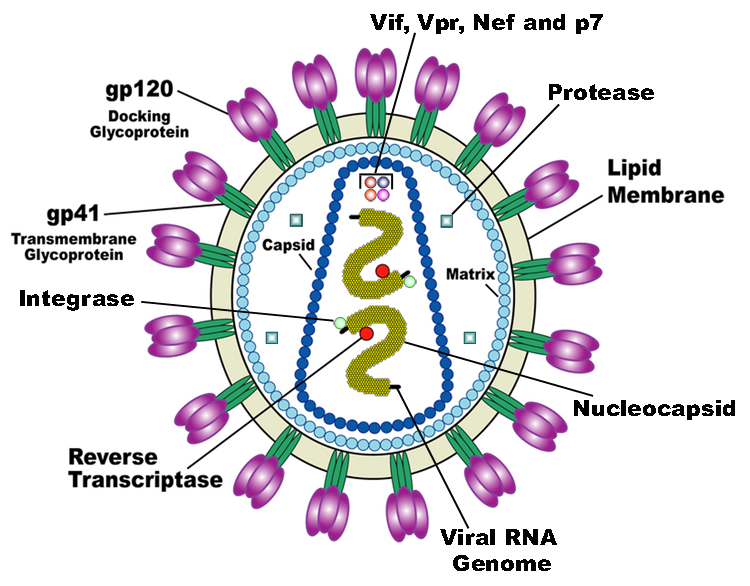
\includegraphics[width=0.85\textwidth]{VirtualScreening/Figures/HIV_Virion-en.png}
  \label{subfig:HIVDiagram}
}
\subfigure[Replication cycle of HIV. Figure reprinted from \citep{296-2010}.]
{
  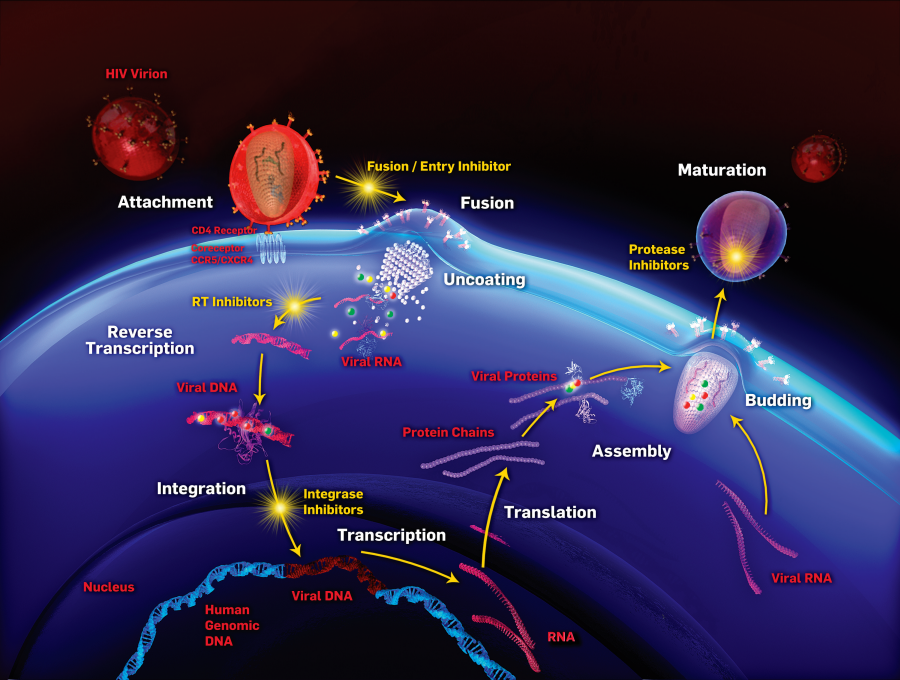
\includegraphics[width=0.85\textwidth]{VirtualScreening/Figures/HIVReplicationCycle.png}
  \label{subfig:HIVReplicationCycle}
}
\caption{Diagram and replication cycle of HIV.}
\label{fig:HIVDiagramAndReplicationCycle}
\end{figure}

Two types of HIV have been characterized, namely HIV-1 and HIV-2. HIV-1 is the virus that was initially discovered. It is more virulent, more infective, and is the cause of the majority of HIV infections globally. In this thesis, all the abbreviations of HIV implicitly refers to HIV-1.

At present, 25 drugs have been approved by US FDA for the treatment of HIV \citep{300-2010}. Among them, TDF is a purine analogue \citep{301-2010} and a potent inhibitor of both HIV RT and HBV RT \citep{165-2008}. Recent scientific studies claimed that a considerably greater proportion of recipients of TDF 300 mg once daily achieves a complete response at week 48 than oral adefovir dipivoxil 10 mg once daily \citep{165-2008}. Such results prove the advantages of TDF over other first-line oral antiviral therapies. TDF is also generally less expensive and more convenient to administer, as it does not require dosing on an empty stomach \citep{159-2009}.

However, clinical feedback shows that TDF exhibits strong side effects (Figure \ref{fig:SideEffect} \citep{658-2011}), causing osteomalacia, mitochondrial toxicity on the renal proximal tubule \citep{185-2006,186-2003}. Justification of side effects shows that
\begin{itemize}
\item S-Adenosyl-L-Homocysteine hydrolase is affected, leading to defect in DNA methylation-dependent gene silencing \citep{182-2005}. TDF shows signs of immunosuppressive activity \citep{183-2007}.
\item Adenosine deaminase is inhibited, resulting in reduced breakdown of adenosine from food and decreased turnover of nucleic acids in tissues \citep{184-2005}. TDF shows signs of hepatic and adrenal toxicity \citep{187-2000}.
\item Purine nucleoside phosphorylase is also inhibited. TDF exhibits toxicity toward T cells \citep{188-1981}.
\end{itemize}

\begin{figure}
\centering
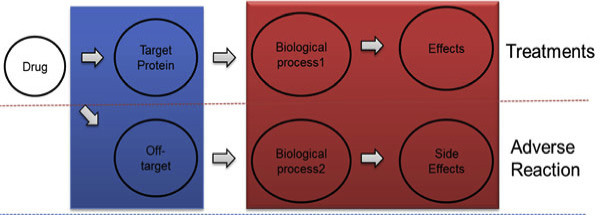
\includegraphics[width=\textwidth]{VirtualScreening/Figures/SideEffect.png}
\caption{Side effects of drugs. Figure reprinted from \citep{658-2011}.}
\label{fig:SideEffect}
\end{figure}

Figure \ref{fig:EnzymaticAssay}, reprinted from Sigma-Aldrich Co., shows the enzymatic assay of the above three enzymes, which break down S-Adenosyl-L-Homocysteine eventually into uric acid inside human bodies. For HIV-infected patients who take TDF as the primary drug, it is unfortunate that these three essential enzymes are simultaneously inhibited by TDF.

\begin{figure}
\centering
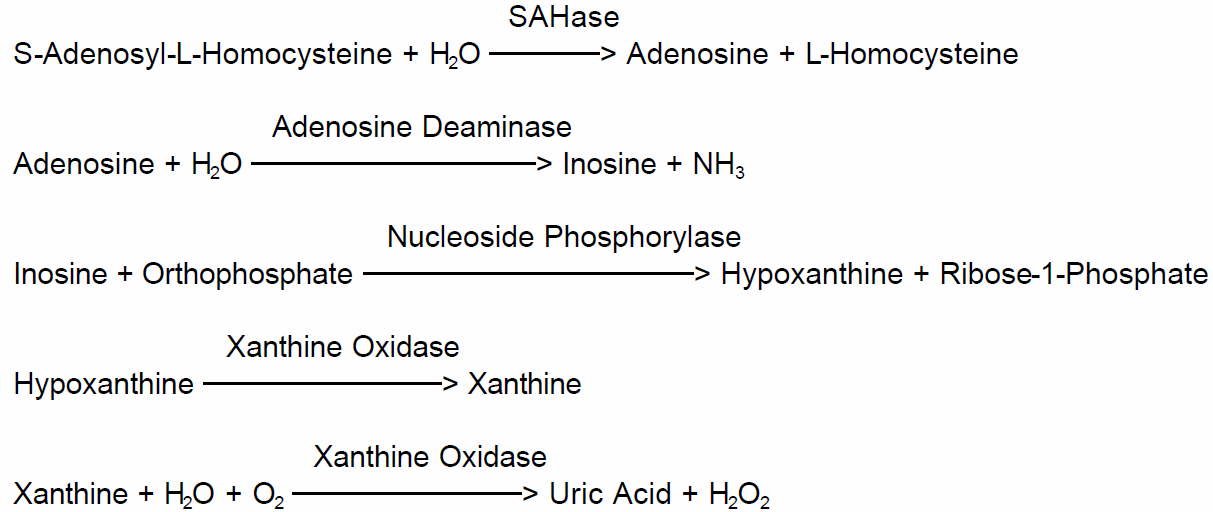
\includegraphics[width=\textwidth]{VirtualScreening/Figures/EnzymaticAssay.png}
\caption{Enzymatic assay of S-Adenosyl-L-Homocysteine hydrolase. Figure reprinted from Sigma-Aldrich Co.}
\label{fig:EnzymaticAssay}
\end{figure}

In addition, TDF is somewhat structurally similar to an inhibitor of S-Adenosylmethionine decarboxylase (AdoMetDC) judging from the querying results of the SEA database \citep{380-2007} using MDL Drug Data Report (MDDR) with two different molecular descriptors, the Scitegic ECFP4 fingerprint and the Daylight fingerprint. Tanimoto coefficient is a similarity metric based on fingerprints. The higher the value, the more similar the compounds are. Table \ref{tab:TanimotoCoefficients} shows that TDF is structurally similar to the inhibitors of SAHH, ADA, PNP, and AdoMetDC, hence TDF is likely to inhibit them in addition to HIV RT.

\begin{table}
\centering
\begin{tabular*}
{\textwidth}
{@{\extracolsep{\fill}}rrr}
\toprule
& Scitegic ECFP4 fingerprint & Daylight fingerprint\\
\midrule
HIV RT inhibitor & 1.00 & 1.00 \\
SAHH inhibitor & 0.51 & 0.70 \\
ADA inhibitor & 0.42 & 0.75 \\
PNP inhibitor & 0.51 & 0.76 \\
AdoMetDC inhibitor & 0.33 & Unknown \\
\bottomrule
\end{tabular*}
\caption{Tanimoto coefficients between TDF and the inhibitors of HIV RT, SAHH, ADA, PNP, and AdoMetDC using the Scitegic ECFP4 and Daylight fingerprints.}
\label{tab:TanimotoCoefficients}
\end{table}

\section{Computational Background}

AutoDock Vina \citep{595-2010} is a competitive docking tool. It's free and open source. It runs faster than its predecessor AutoDock4 \citep{596-2009} by an order of magnitude \citep{556-2010}. Released in 2010, Vina has been cited by 117 other publications and adopted by many researchers \citep{609-2010}.

Figure \ref{fig:VinaInputOutput} shows the input and output of Vina. The input to Vina is threefold, including a receptor, a ligand, and a box. The output from Vina is twofold, including predicted conformations and their predicted free energy in kcal/mol. The receptor is usually a target protein for the single ligand to dock against, and the box is used to restrict the search space, i.e. the conformational space for the ligand to translate and rotate inside.

\begin{figure}
\centering
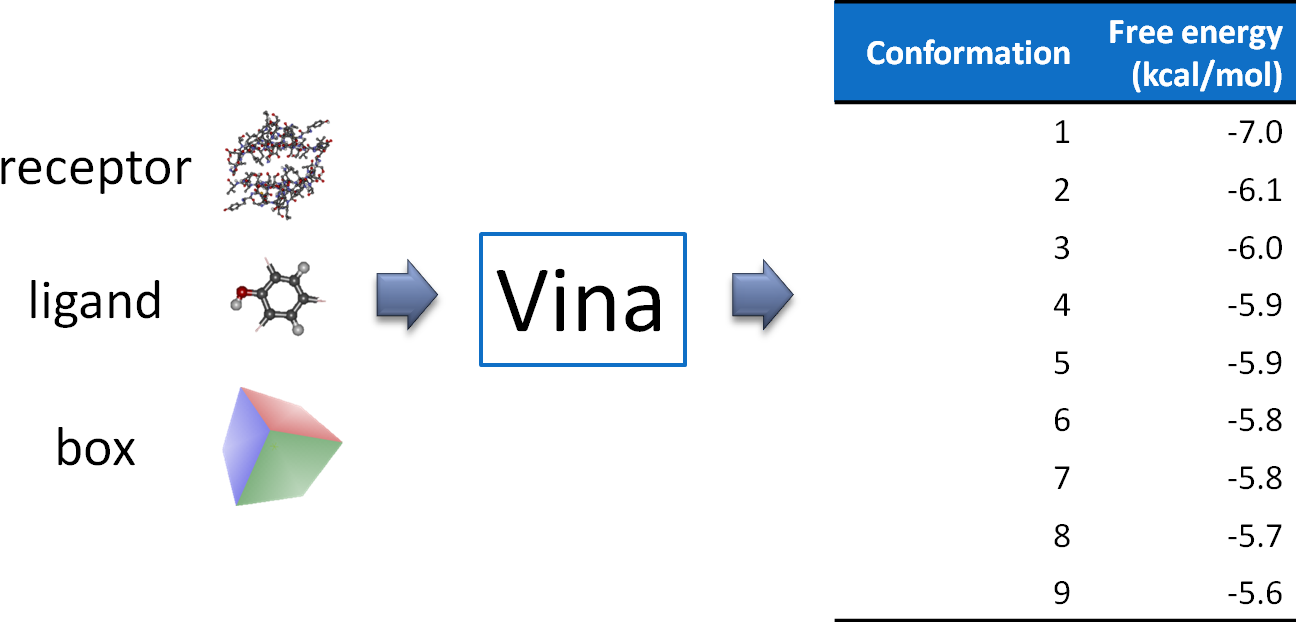
\includegraphics[width=\textwidth]{VirtualScreening/Figures/VinaInputOutput.png}
\caption{Input and output of AutoDock Vina.}
\label{fig:VinaInputOutput}
\end{figure}

Vina consists of two basic components, a scoring function to predict the binding affinity, and an algorithm to explore the conformational space of the ligand.

\subsection{Scoring Function}
\label{sec:VinaScoringFunction}

The scoring function of Vina is inspired by XScore \citep{573-2002} and is tuned with PDBbind \citep{529-2004,530-2005} by linear regression. It is made up of a conformation-dependent part and a conformation-independent part. The conformation-dependent part is a weighted linear sum of five terms over all the pairs of atom $i$ and atom $j$ that can move relative to each other. It is calculated from equation \eqref{eqn:ScoringFunction} where $t_i$ and $t_j$ are the XScore atom types of $i$ and $j$ respectively, and $r_{ij}$ is their interatomic distance. The five terms are calculated from equations \eqref{eqn:Gauss1} to \eqref{eqn:HydrogenBonding} where $d_{ij}$ is the surface distance calculated from equation \eqref{eqn:SurfaceDistance} and defined as the interatomic distance minus the sum of van der Waals radius (Figure \ref{fig:DockingDistance}).

\begin{eqnarray}
\label{eqn:ScoringFunction}
e = \sum_{i < j} &\Big(&(-0.035579) * Gauss_1(t_i, t_j, r_{ij}) + \nonumber \\
&&(-0.005156) * Gauss_2(t_i, t_j, r_{ij}) + \nonumber \\
&&(+0.840245) * Repulsion(t_i, t_j, r_{ij}) + \nonumber \\
&&(-0.035069) * HydrophobicInteraction(t_i, t_j, r_{ij}) + \nonumber \\
&&(-0.587439) * HydrogenBonding(t_i, t_j, r_{ij})\Big)
\end{eqnarray}

\begin{equation}
\label{eqn:Gauss1}
Gauss_1(t_i, t_j, r_{ij}) = e^{-(d_{ij} / 0.5)^2}
\end{equation}
\begin{equation}
\label{eqn:Gauss2}
Gauss_2(t_i, t_j, r_{ij}) = e^{-((d_{ij} - 3) / 2)^2}
\end{equation}
\begin{equation}
\label{eqn:Repulsion}
Repulsion(t_i, t_j, r_{ij}) =
\begin{cases}
d_{ij}^2 & \text{if } d_{ij} < 0\\
0 &\text{if } d_{ij} \geq 0
\end{cases}
\end{equation}
\begin{equation}
\label{eqn:HydrophobicInteraction}
HydrophobicInteraction(t_i, t_j, r_{ij}) =
\begin{cases}
1 & \text{if } d_{ij} \leq 0.5\\
1.5 - d_{ij} & \text{if } 0.5 < d_{ij} < 1.5\\
0 & \text{if } d_{ij} \geq 1.5\\
\end{cases}
\end{equation}
\begin{equation}
\label{eqn:HydrogenBonding}
HydrogenBonding(t_i, t_j, r_{ij}) =
\begin{cases}
1 & \text{if } d_{ij} \leq -0.7\\
d_{ij} / (-0.7) & \text{if } -0.7 < d_{ij} < 0\\
0 & \text{if } d_{ij} \geq 0\\
\end{cases}
\end{equation}

\begin{equation}
\label{eqn:SurfaceDistance}
d_{ij} = r_{ij} - (R_{t_i} + R_{t_j})
\end{equation}

\begin{figure}
\centering
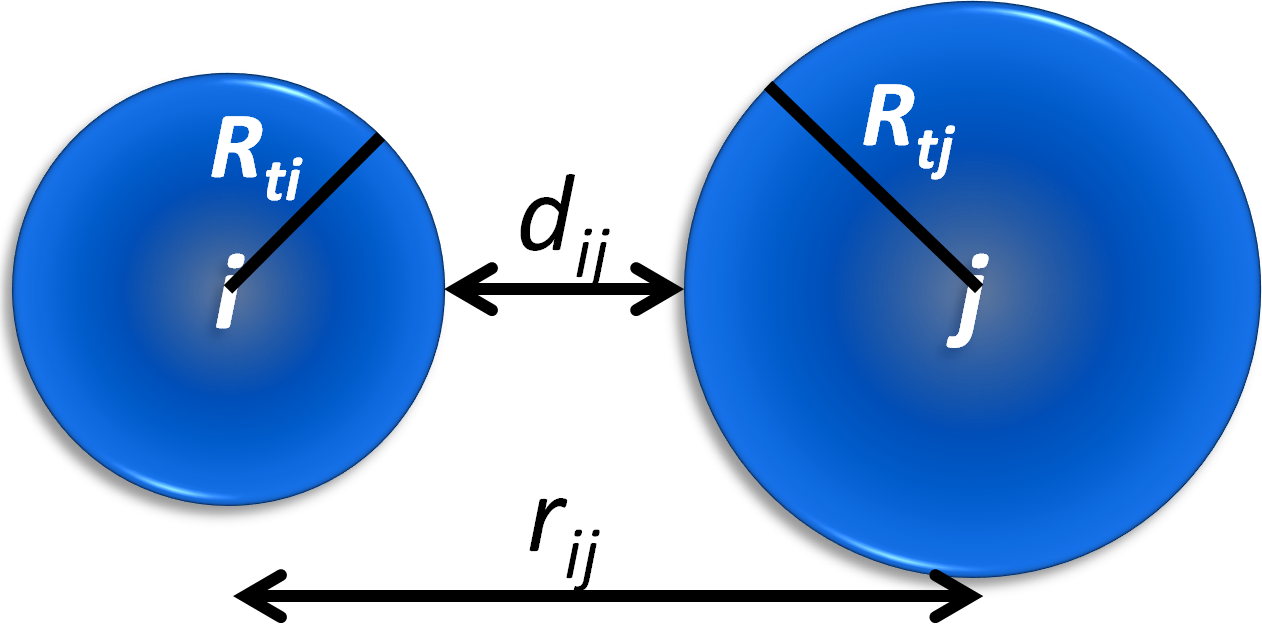
\includegraphics[width=\textwidth]{VirtualScreening/Figures/Distance.png}
\caption{Visualization of interatomic distance and surface distance.}
\label{fig:DockingDistance}
\end{figure}

In Vina, all the five terms are cut off at $r_{ij}$ = 8 \AA. Figure \ref{fig:ScoringFunction} \citep{595-2010} plots three combinations of weighted scoring function terms. The steric interactions refers to the first three terms. The optimization algorithm attempts to find the global minimum of $e$ and other low-scoring conformations, which it then ranks.

\begin{figure}[t]
\centering
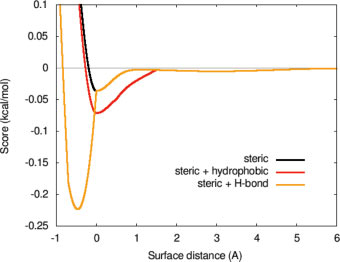
\includegraphics[width=\textwidth]{VirtualScreening/Figures/ScoringFunction.png}
\caption{Weighted scoring function term combinations. Figure reprinted from \citep{595-2010}.}
\label{fig:ScoringFunction}
\end{figure}

The conformation-dependent part can be seen as the sum of intermolecular and intramolecular contributions. It is calculated from equation \eqref{eqn:inter-intra} where $e_{inter}$ is the summation over all the heavy atoms between receptor and ligand, and $e_{intra}$ is the summation over all the ligand heavy atoms that are separated by three consecutive covalent bonds and can move relative to each other.
\begin{equation}
\label{eqn:inter-intra}
e = e_{inter} + e_{intra}
\end{equation}

The conformation-independent part penalizes $e_{inter}$ for ligand flexibility and the predicted free energy of conformation $k$ for output, denoted as $e'_k$, is calculated from equation \eqref{eqn:FlexibilityPenalty} where $k$ is the subscript for conformation, $e_{intra,1}$ is the $e_{intra}$ of the first, i.e. lowest-scoring conformation, $N_{Active Torsions}$ is the number of active torsions and $N_{InactiveTorsions}$ is the number of inactive torsions. Note that $e_{intra,1}$, rather than $e_{intra,k}$, acts as subtrahend in order to preserve the ranking.
\begin{equation}
\label{eqn:FlexibilityPenalty}
e'_k = \frac{e_k - e_{intra,1}}{1 + 0.05846 * (N_{ActiveTorsions} + 0.5 * N_{InactiveTorsions})}
\end{equation}

The scoring function is basically a function of three variables, $t_i$, $t_j$, and $r_{ij}$. These three variables have both a known lower bound and a known upper bound, so it is possible to precalculate the value of the scoring function by approximation. On one hand, since there are only 17 XScore atom types, there are 17 * 18 / 2 = 153 possible combinations of $t_i$ and $t_j$. On the other hand, since $r_{ij}$ is cut off at 8 \AA, it is possible for Vina to divide the range [0, 8] into 2,048 segments. In fact, Vina precalculates the scoring function for each of the 153 possible combinations of $t_i$ and $t_j$ and for each of the 2,048 possible values of $r_{ij}$, and a score is approximated by linearly interpolating the two nearest precalculated values.

In most cases, the receptor is rigid. For the sake of fast evaluation of $e_{inter}$, grid maps are often built. A grid map of atom type \textit{t} is constructed by placing virtual probe atoms of atom type \textit{t} along the X, Y, and Z dimensions of the search box at a certain granularity (Figure \ref{fig:GridMap}). The $e_{inter}$ value of a ligand atom can be approximated by linear interpolation of the precalculated $e_{inter}$'s of its eight corner probe atoms. In Vina, the grid map granularity is hard coded to be 0.375 \AA.

\begin{figure}[h!]
\centering
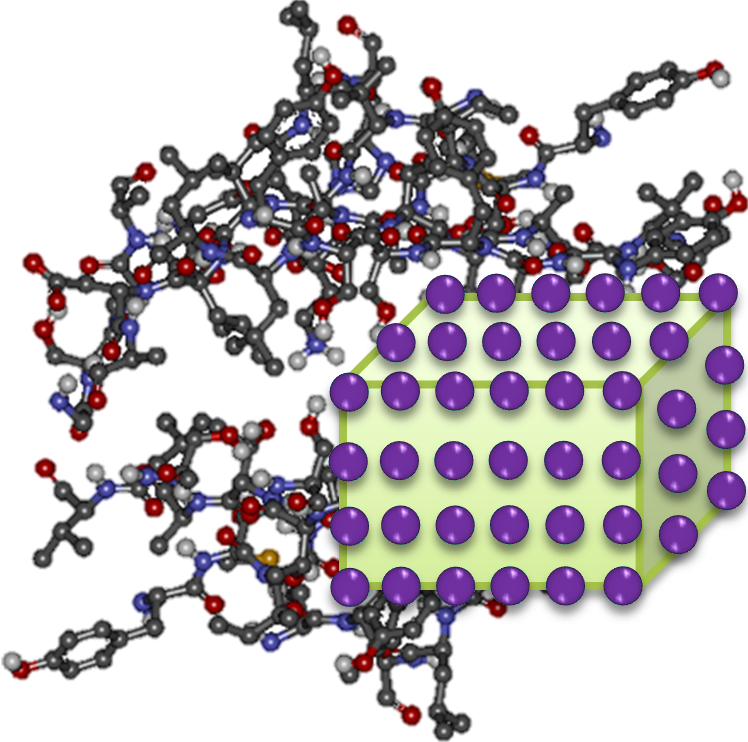
\includegraphics[width=\textwidth]{VirtualScreening/Figures/GridMap.png}
\caption{Grid map for fast evaluation of $e_{inter}$. Probe atoms are shown in purple.}
\label{fig:GridMap}
\end{figure}

\subsection{Optimization Algorithm}

According to Vina's original paper \citep{595-2010}, several stochastic algorithms had been tested, including genetic algorithm, particle swarm optimization, and simulated annealing. Finally its authors settled on Monte Carlo algorithm for global optimization and the Broyden-Fletcher-Goldfarb-Shanno (BFGS) \citep{786-2006} algorithm for local optimization.

\begin{figure}
\centering
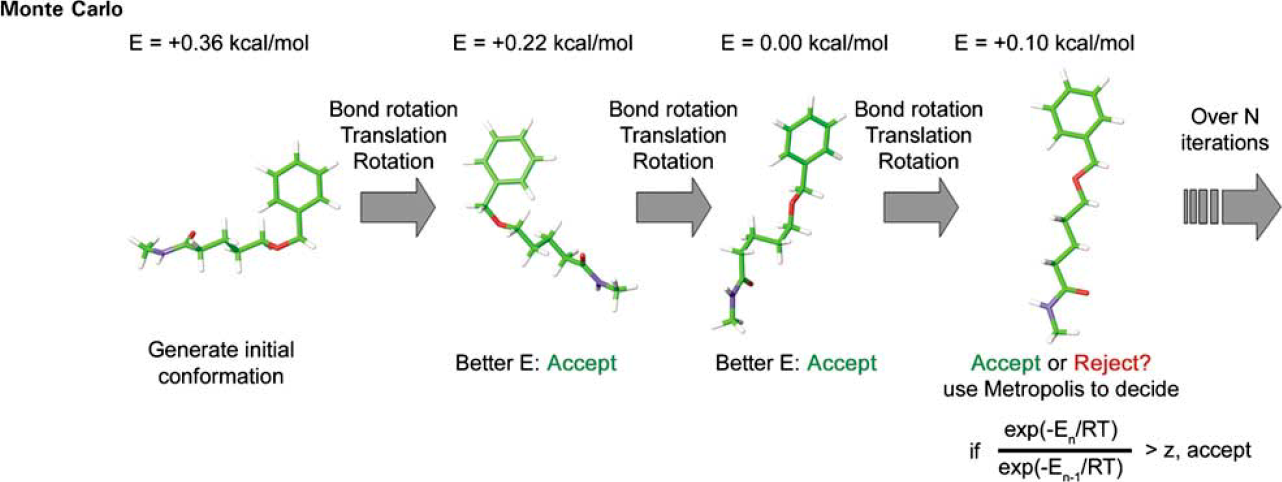
\includegraphics[width=\textwidth]{VirtualScreening/Figures/MonteCarlo.png}
\caption{Monte Carlo algorithm for molecular docking. Figure reprinted from \citep{493-2008}.}
\label{fig:DockingByMonteCarlo}
\end{figure}

In Vina, a succession of steps consisting of a mutation and a BFGS local optimization are taken, with each step being accepted according to the Metropolis criterion (Figure \ref{fig:DockingByMonteCarlo} \citep{493-2008}). BFGS is a kind of quasi-Newton optimization methods. It approximates the inverse Hessian matrix, and uses not only the value of the scoring function but also its gradient, which are the derivatives of the scoring function with respect to the position and orientation of the ligand, and the torsions for the active rotatable bonds in the ligand. BFGS involves three major steps. It first derives a descent direction from the approximated inverse Hessian matrix, then derives a step length along the descent direction from line search, and updates the approximation of inverse Hessian matrix. These three steps are repeated iteratively until an estimated number of iterations are done.

Multithreading is achieved by concurrently running multiple independent Monte Carlo tasks starting from random initial conformations. Figure \ref{fig:VinaThreadProfile} shows the thread profile of one run of Vina on a 4-core computer. The main thread, thread 3176, managed the program startup and cleanup. Four workers threads, distributed across four physical cores, actually executed the parallel Monte Carlo tasks.

\begin{figure}
\centering
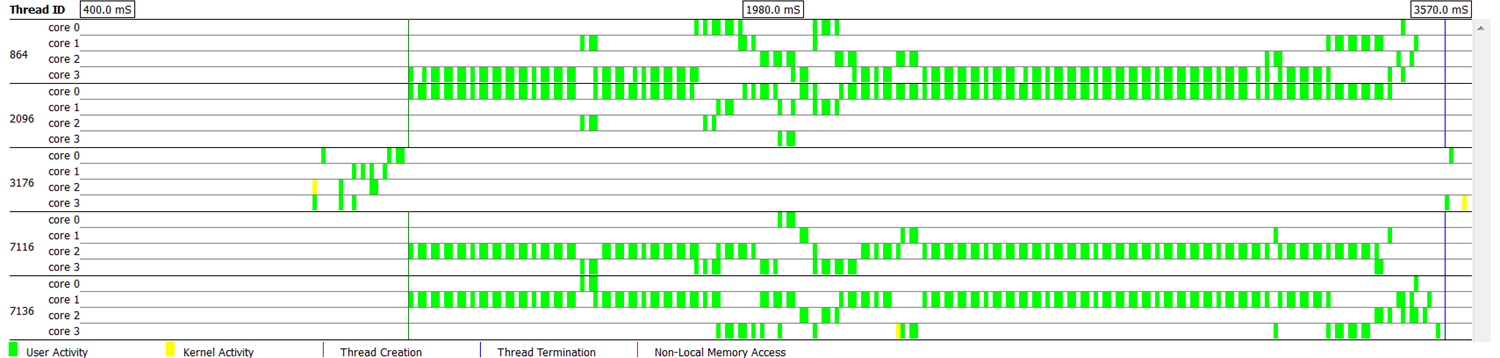
\includegraphics[width=\textwidth]{VirtualScreening/Figures/ThreadProfile.png}
\caption{Thread profile of AutoDock Vina.}
\label{fig:VinaThreadProfile}
\end{figure}

\section{Method}

We developed a fast virtual screening tool called idock, and used it for the discovery of compounds that inhibit HIV RT without affecting SAHH, ADA, PNP, or AdoMetDC. idock borrows many great ideas from Vina, and meanwhile introduces its own innovations.

Figure \ref{fig:idockFlowchart} shows the overall flowchart of idock. During initialization, idock approximates the scoring function by precalculating it for all the possible combinations of XScore atom types and distances. It then parses the receptor and determines the XScore atom types with the aid of residue sequences. It then creates a thread pool to hold reusable threads. It then fetches a ligand, if any, from a user-specified folder to perform docking. It parses the ligand and automatically detects inactive torsions. It then builds grid maps of granularity 0.15625 \AA by default on the fly by multithreading. It then schedules multiple Monte Carlo tasks to the thread pool for concurrent execution. It then merges conformations found by separate threads and clusters them with RMSD 2.0 \AA. Finally it dumps the conformations to the user-specified output folder and displays the predicted free energy on screen.

\begin{figure}
\centering
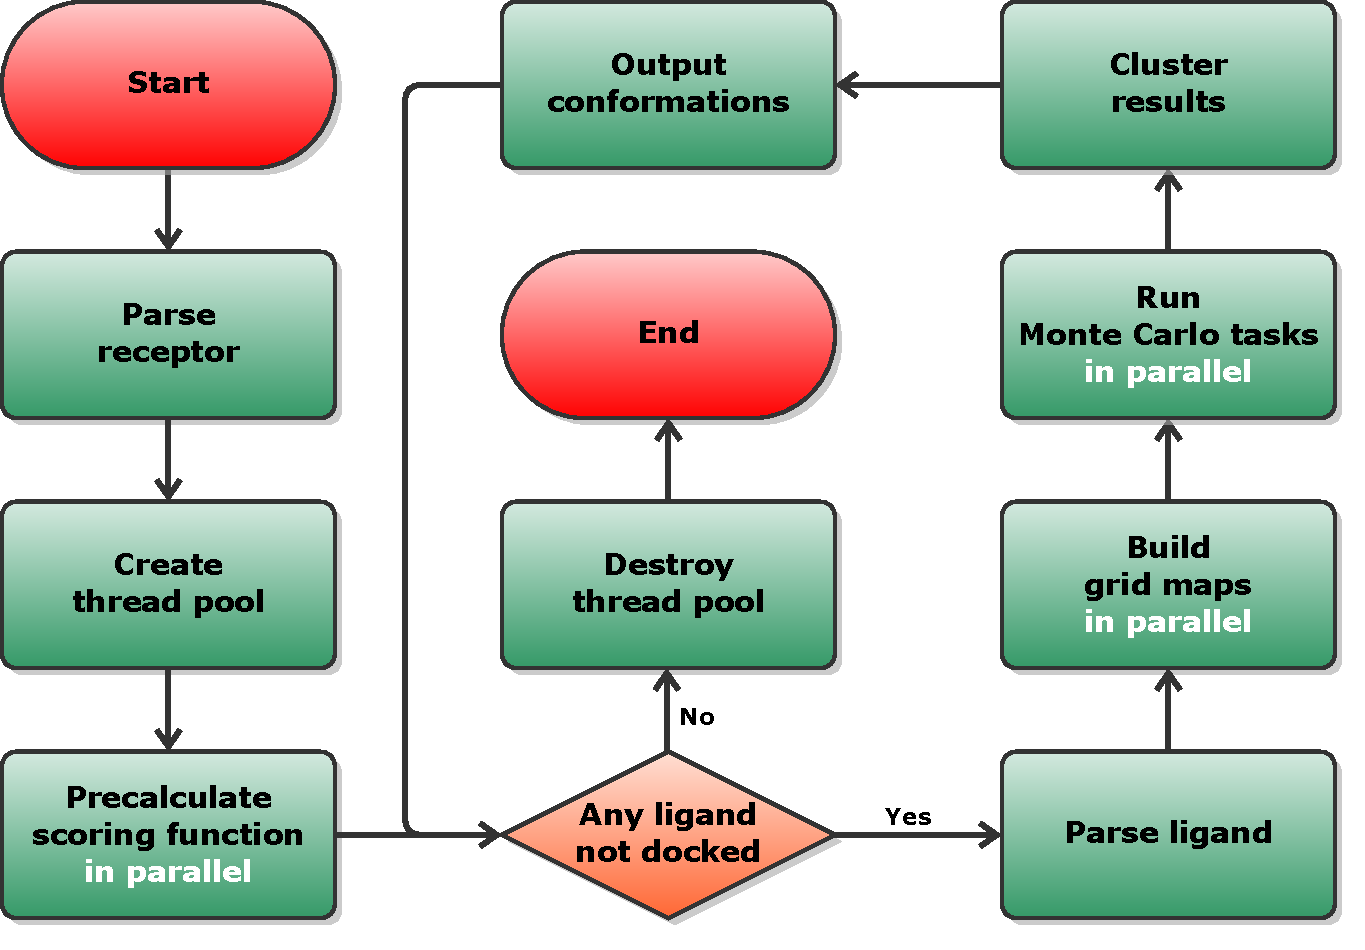
\includegraphics[width=\textwidth]{VirtualScreening/Figures/Flowchart.pdf}
\caption{Flowchart of idock.}
\label{fig:idockFlowchart}
\end{figure}

\subsection{Scoring Function}

idock inherits from Vina the scoring function as described in section \ref{sec:VinaScoringFunction}, except that it splits [0, 8], the value range of $r_{ij}$, into 16,384 segments instead of 2,048 in Vina, resulting in an absolute approximation error of merely 0.002 kcal/mol on average (Figure \ref{fig:ScoringFunctionApproximationAbsoluteError}). Due to a higher density of segments, idock substitutes direct assignment for linear interpolation for fast evaluation of scoring function at the cost of a little bit longer precalculation time.

\begin{figure}
\centering
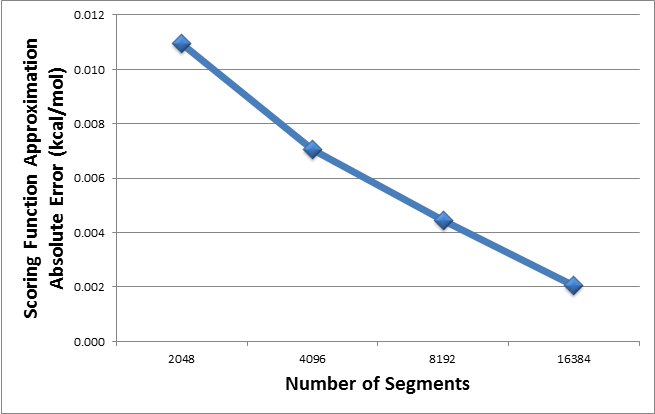
\includegraphics[width=\textwidth]{VirtualScreening/Figures/ScoringFunctionApproximationAbsoluteError.png}
\caption{Scoring function approximation absolute error against segments.}
\label{fig:ScoringFunctionApproximationAbsoluteError}
\end{figure}

In idock, grid map granularity is exposed to be an optional program argument with a default value of 0.15625 \AA. Likewise, due to a higher density of probe atoms, idock substitutes direct assignment for linear interpolation for fast evaluation of $e_{inter}$ at the cost of longer precalculation time and larger memory storage (Figure \ref{fig:GridMapStorage}). Therefore, the creation of grid maps is carried out on the fly when necessary and abstracted into tasks, which are then distributed to the thread pool for concurrent execution.

\begin{figure}
\centering
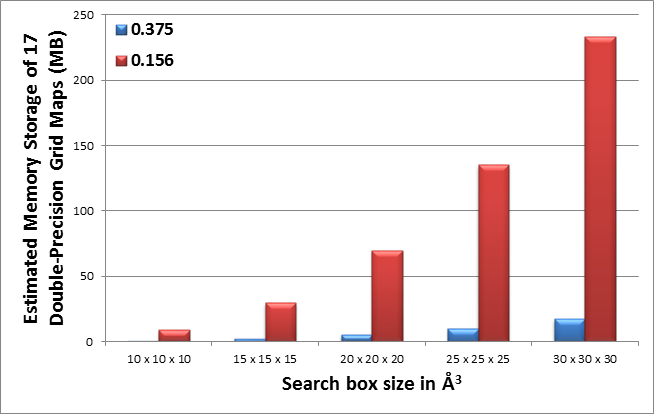
\includegraphics[width=\textwidth]{VirtualScreening/Figures/GridMapStorage.png}
\caption{Estimated memory storage of 17 double-precision grid maps of granularities 0.375 \AA and 0.15625 \AA against search box size.}
\label{fig:GridMapStorage}
\end{figure}

\subsection{Inactive Torsions}

idock automatically detects inactive torsions, which are presented and activated in the input file in pdbqt format but have no impact on the overall scoring, such as \textemdash{OH} and \textemdash{NH$_2$}, because they only rotate the hydrogens. Figure \ref{fig:InactiveTorsions} shows ZINC00572984, which contains 4 active torsions defined by the python script \textit{prepare\_ligand4.py} provided by AutoDock Tools \citep{785-1999,596-2009}, but two of them, highlighted in yellow, will be deactivated while being parsed in idock. This kind of automatic deactivation of inactive torsions reduces the dimension of variables to optimize in the local optimization step.

\begin{figure}
\centering
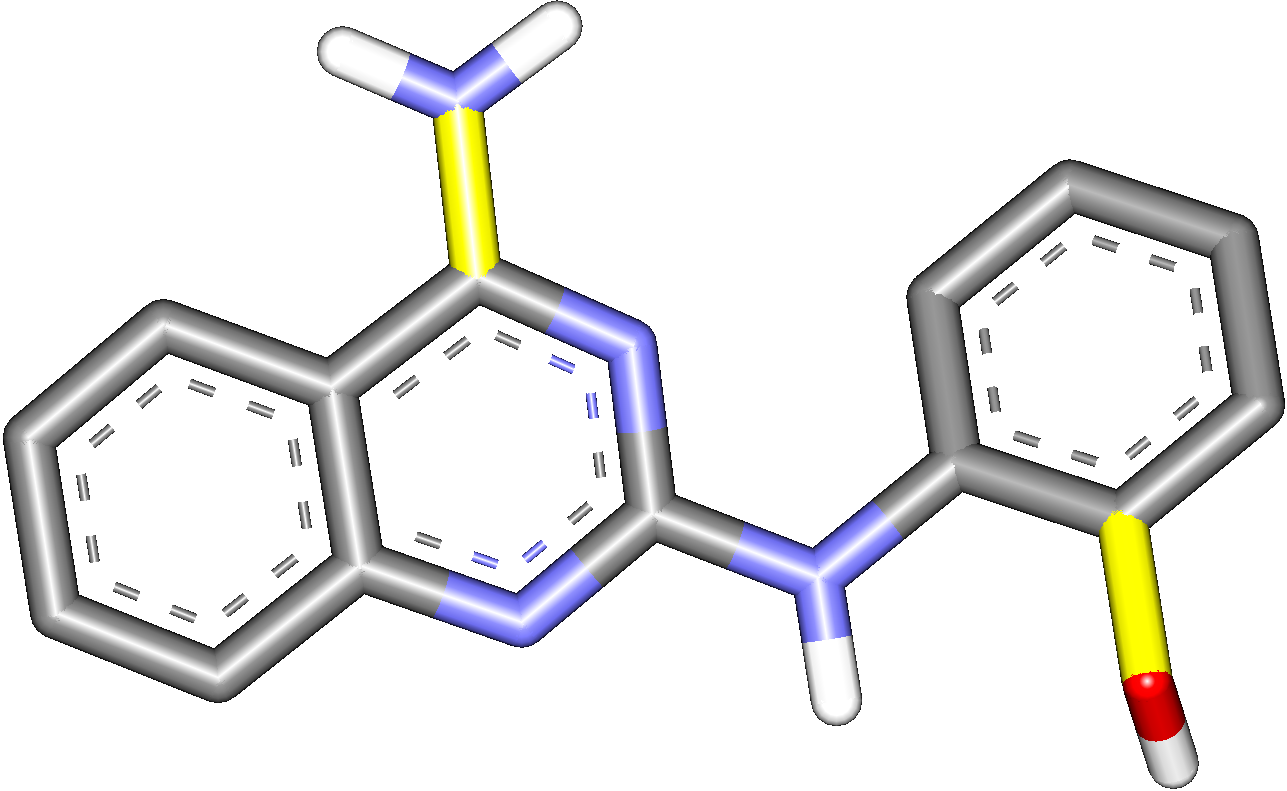
\includegraphics[width=\textwidth]{VirtualScreening/Figures/ZINC00572984.png}
\caption{Example of inactive torsions highlighted in yellow. Nonpolar hydrogens are not shown for clarity.}
\label{fig:InactiveTorsions}
\end{figure}

\subsection{Optimization Algorithm}

idock also inherits from Vina the Monte Carlo algorithm for global optimization and the BFGS algorithm for local optimization, except that the Monte Carlo iterations are far fewer and the BFGS iterations are more. On one hand, the fewer number of Monte Carlo iterations is compensated by a larger number of parallel Monte Carlo tasks, which is 64 by default in idock compared to 8 in Vina, guaranteeing better conformation diversity and higher CPU utilization on many-core computers. On the other hand, the BFGS stopping criterion does not depend on an estimated number of iterations, which is the case in Vina, but depends on the outcome of line search. The BFGS local optimization stops if and only if no appropriate step length can be obtained by line search.

\subsection{C++ Implementation Tricks}

idock implements its own thread pool in order to reuse threads and maintain a high CPU utilization throughout the entire screening procedure. The thread pool parallelizes the creation of grid maps and the execution of Monte Carlo tasks. idock estimates the capacity of every vector structure and intensively utilizes Rvalue reference, a new feature in the C++0x standard, to avoid frequent memory reallocation. In order to efficiently represent root and branch frames of the ligand, idock flattens Vina's tree-like recursive data structure into simple linear array structure to ensure a high data cache hit rate and easy coding. idock accelerates the assignment of XScore atom types by making use of residue information for receptor and branch information for ligand, without detecting covalent bonds among atoms.

\section{Data}

\subsection{Proteins}

Crystal structures of HIV RT, SAHH, ADA, PNP, and AdoMetDC were collected from the Protein Data Bank (PDB) database \citep{540-2000,539-2000,537-2003,105-2007,538-2008}. Protein-ligand complexes with PDB IDs of 2ZD1, 1LI4, 3IAR, 3BGS, and 3H0W were selected because 1) they are human enzymes, 2) their chains are long enough for scientific analysis, and 3) they were crystallized at high resolutions (Table \ref{tab:SelectedPDBEntries}).

\begin{table}[h]
\centering
\begin{tabular*}
{\textwidth}
{@{\extracolsep{\fill}}cccccc}
\toprule
PDB ID & Protein & Chain & Length & Resolution & Ligand \\
\midrule
2ZD1 & HIV RT      & A, B & 557, 428 & 1.80 \AA & T27 \\
1LI4   & SAHH       & A     & 432        & 2.01 \AA & NAD \\
3IAR  & ADA         & A     & 367         & 1.52 \AA & 3D1 \\
3BGS  & PNP         & A     & 289         & 2.10 \AA & DIH \\
3H0W & AdoMetDC & A, B & 266, 67   & 1.81 \AA & N8M \\
\bottomrule
\end{tabular*}
\caption{Selected PDB entries of HIV RT, SAHH, ADA, PNP, and AdoMetDC.}
\label{tab:SelectedPDBEntries}
\end{table}

The five proteins were manually extracted from the five complexes downloaded from PDB. The python script \textit{prepare\_receptor4.py} provided by AutoDock Tools \citep{785-1999,596-2009} was then used to remove water molecules, add polar hydrogens, assign AutoDock4 atom types, and convert from pdb format into pdbqt format. Search spaces were then manually defined in cuboid shape to be large enough for ligands to translate and rotate freely (Table \ref{tab:DockingSearchSpaces}).

\begin{table}
\centering
\begin{tabular*}
{\textwidth}
{@{\extracolsep{\fill}}cccc}
\toprule
PDB ID & Protein & Box center (\AA) & Box size (\AA) \\
\midrule
2ZD1 & HIV RT      & (49.712, -28.923, 36.824)  & (18, 18, 20) \\
1LI4   & SAHH       & (35.630, -12.231, 104.708) & (26, 24, 18) \\
3IAR  & ADA          & (8.135, -3.503, -0.112)      & (22, 16, 16) \\
3BGS & PNP           & (15.157, 11.025, 58.157)   & (18, 18, 20) \\
3H0W & AdoMetDC & (-17.359, -7.869, 5.645)    & (20, 16, 18) \\
\bottomrule
\end{tabular*}
\caption{Search spaces in cuboid shape of HIV RT, SAHH, ADA, PNP, and AdoMetDC.}
\label{tab:DockingSearchSpaces}
\end{table}

\subsection{Ligands}

10,928 ligands were collected from the clean drug like subset of ZINC database \citep{532-2005}. These ligands satisfy Lipinski's \textit{Rule of Five} \citep{169-1997,167-2000,168-2004} with LogP value of at most 5, molecular weight between 150 Da and 500 Da, at most 5 hydrogen bond donors, and at most 10 hydrogen bonds acceptors.

The python script \textit{prepare\_ligand4.py} provided by AutoDock Tools \citep{785-1999,596-2009} was used to batch define rotatable bonds and convert the ligands from mol2 format into pdbqt format.

\section{Experiments and Results}

The experiments include 1) validation of both programs to ensure they are suitable for docking ligands against the five proteins, and 2) comparison of their virtual screening performance in terms of execution time, memory usage, predicted free energy, and predicted conformations.

AutoDock Vina \citep{595-2010} x86 version 1.1.2 and idock x86\_64 version 1.0, the most recent versions of both programs at the moment this thesis was composed, were used for virtual screening. Both programs were run on desktop computers with Intel Xeon Dual Quad Core 2.4GHz and 32GB RAM under Ubuntu 10.04.1 x86\_64. The CPU supports Intel's Hyper-Threading technology, so each computer consisting of 8 physical cores can execute 16 logical threads simultaneously.

\subsection{Program Validation}

The five crystal ligands were conformationally randomized and redocked against their proteins by the two programs. Figures \ref{fig:2ZD1-T27} to \ref{fig:3H0W-N8M} show the five proteins in complex with their corresponding crystal and docked ligands. The ligands rendered in green are the crystal ones, the ligands rendered in red are the ones docked by Vina, and the ligands rendered in blue are the ones docked by idock. Table \ref{tab:RMSD} shows the root mean square deviations (RMSDs) between the docked the crystal conformations. The RMSDs are all below 2.0 \AA, a publicly accepted positive control for correct bound structure prediction, indicating both programs are suitable for docking ligands against the five proteins. It should also be noted that the RMSDs obtained by Vina are a little bit better than the ones obtained by idock, especially for the case of PNP. This is probably due to the coarse estimation of intra-ligand free energy in idock, which does not form covalent bonds internally but simply relies on rotatable bonds to detect mobility.

\begin{figure}
\centering
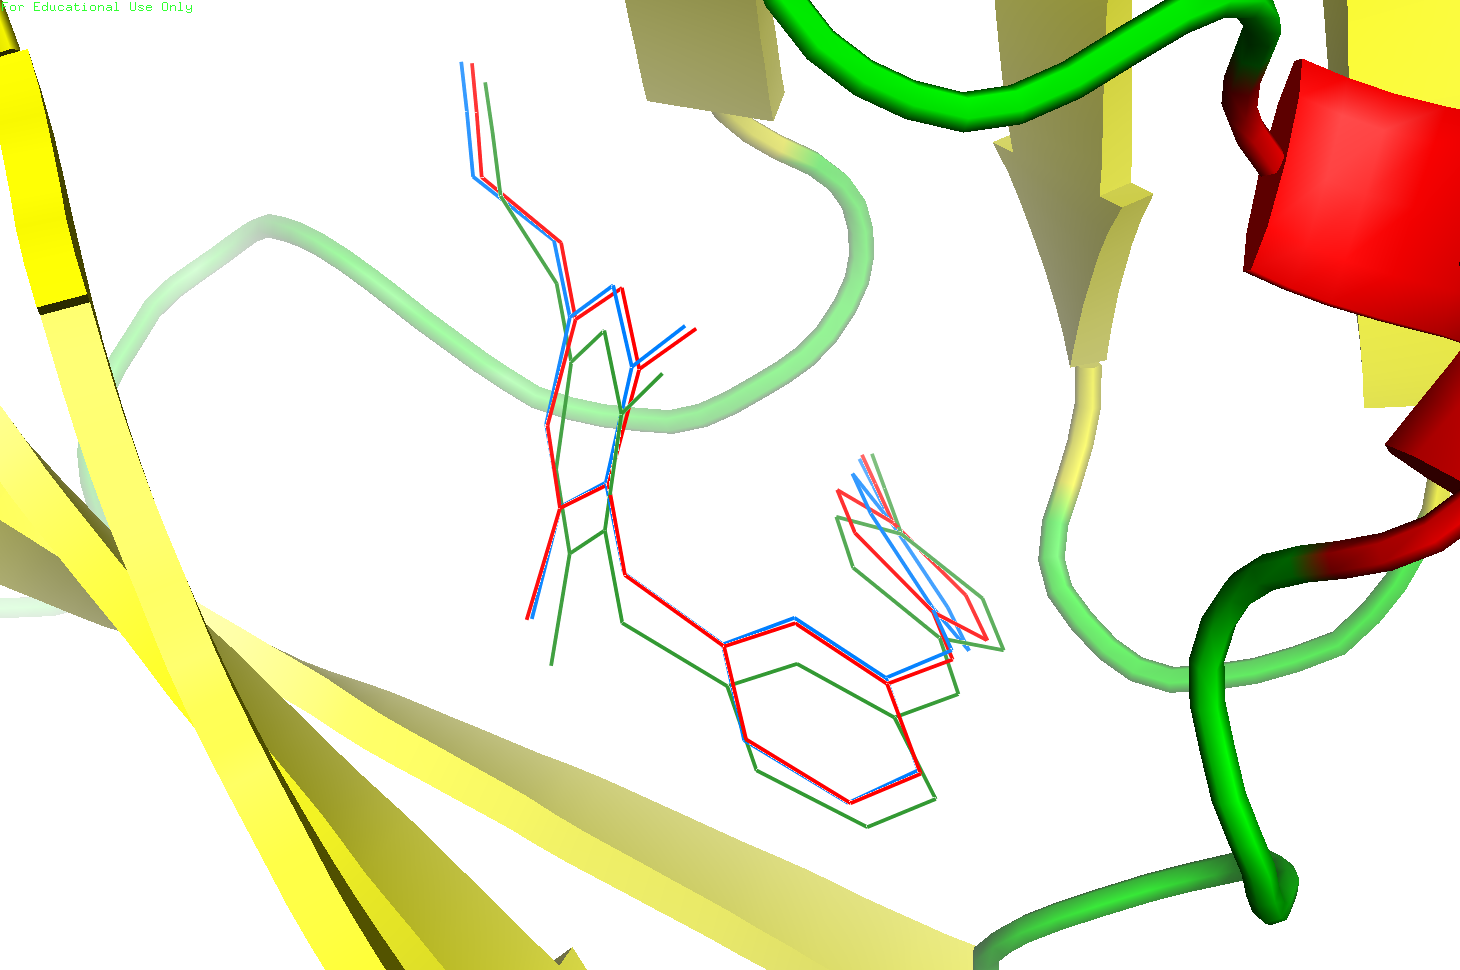
\includegraphics[width=\textwidth]{VirtualScreening/Figures/2ZD1-T27.png}
\caption{HIV RT in complex with crystal and docked T27.}
\label{fig:2ZD1-T27}
\end{figure}

\begin{figure}
\centering
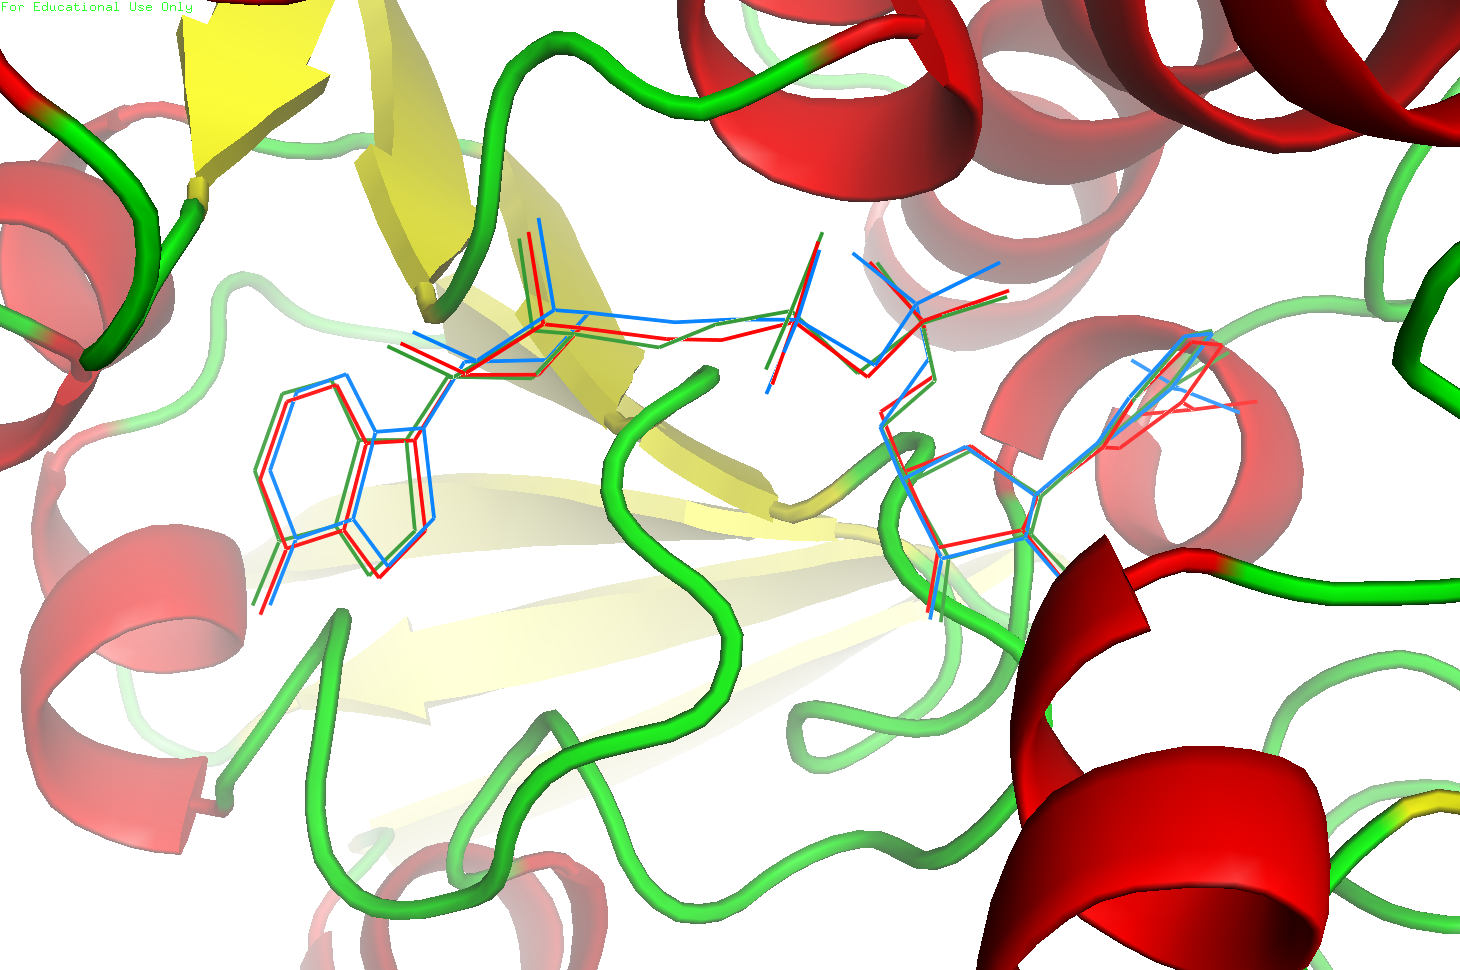
\includegraphics[width=\textwidth]{VirtualScreening/Figures/1LI4-NAD.png}
\caption{SAHH in complex with crystal and docked NAD.}
\label{fig:1LI4-NAD}
\end{figure}

\begin{figure}
\centering
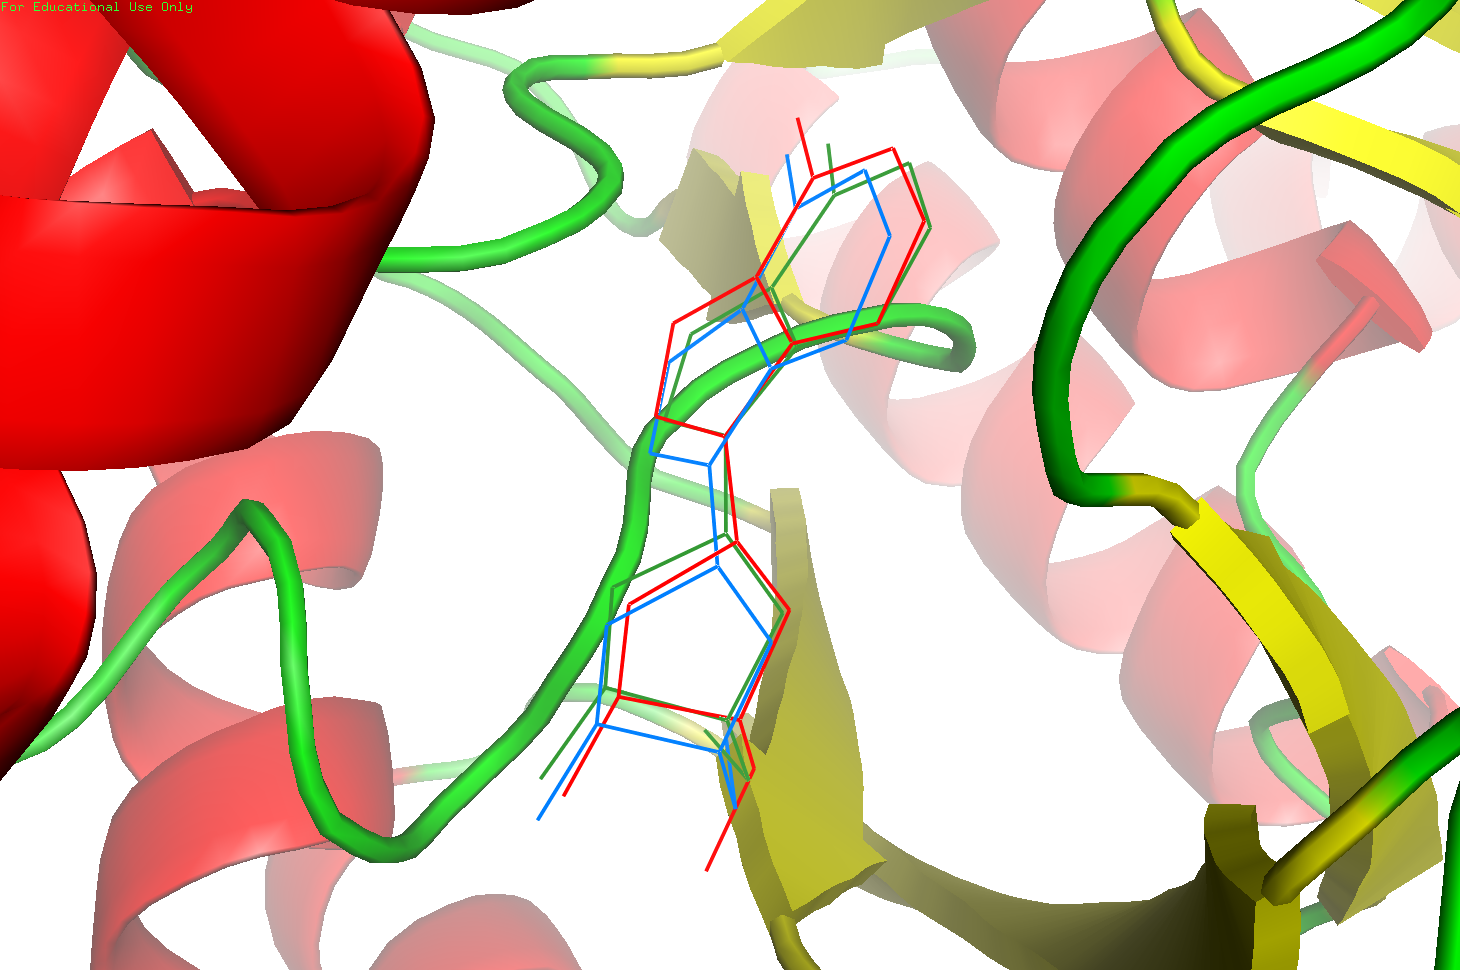
\includegraphics[width=\textwidth]{VirtualScreening/Figures/3IAR-3D1.png}
\caption{ADA in complex with crystal and docked 3D1.}
\label{fig:3IAR-3D1}
\end{figure}

\begin{figure}
\centering
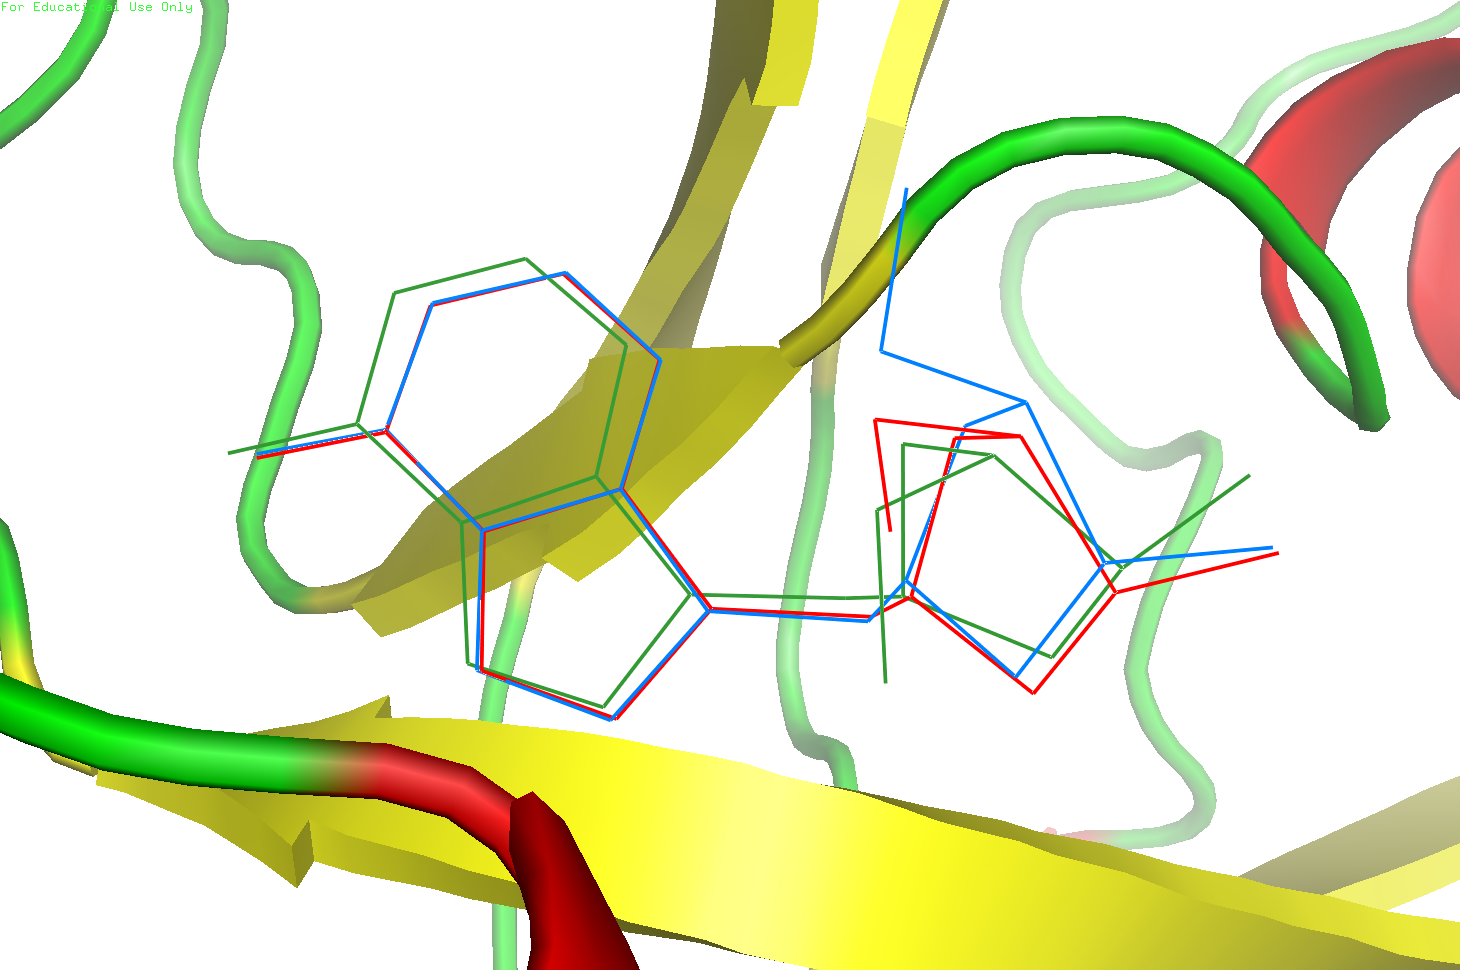
\includegraphics[width=\textwidth]{VirtualScreening/Figures/3BGS-DIH.png}
\caption{PNP in complex with crystal and docked DIH.}
\label{fig:3BGS-DIH}
\end{figure}

\begin{figure}
\centering
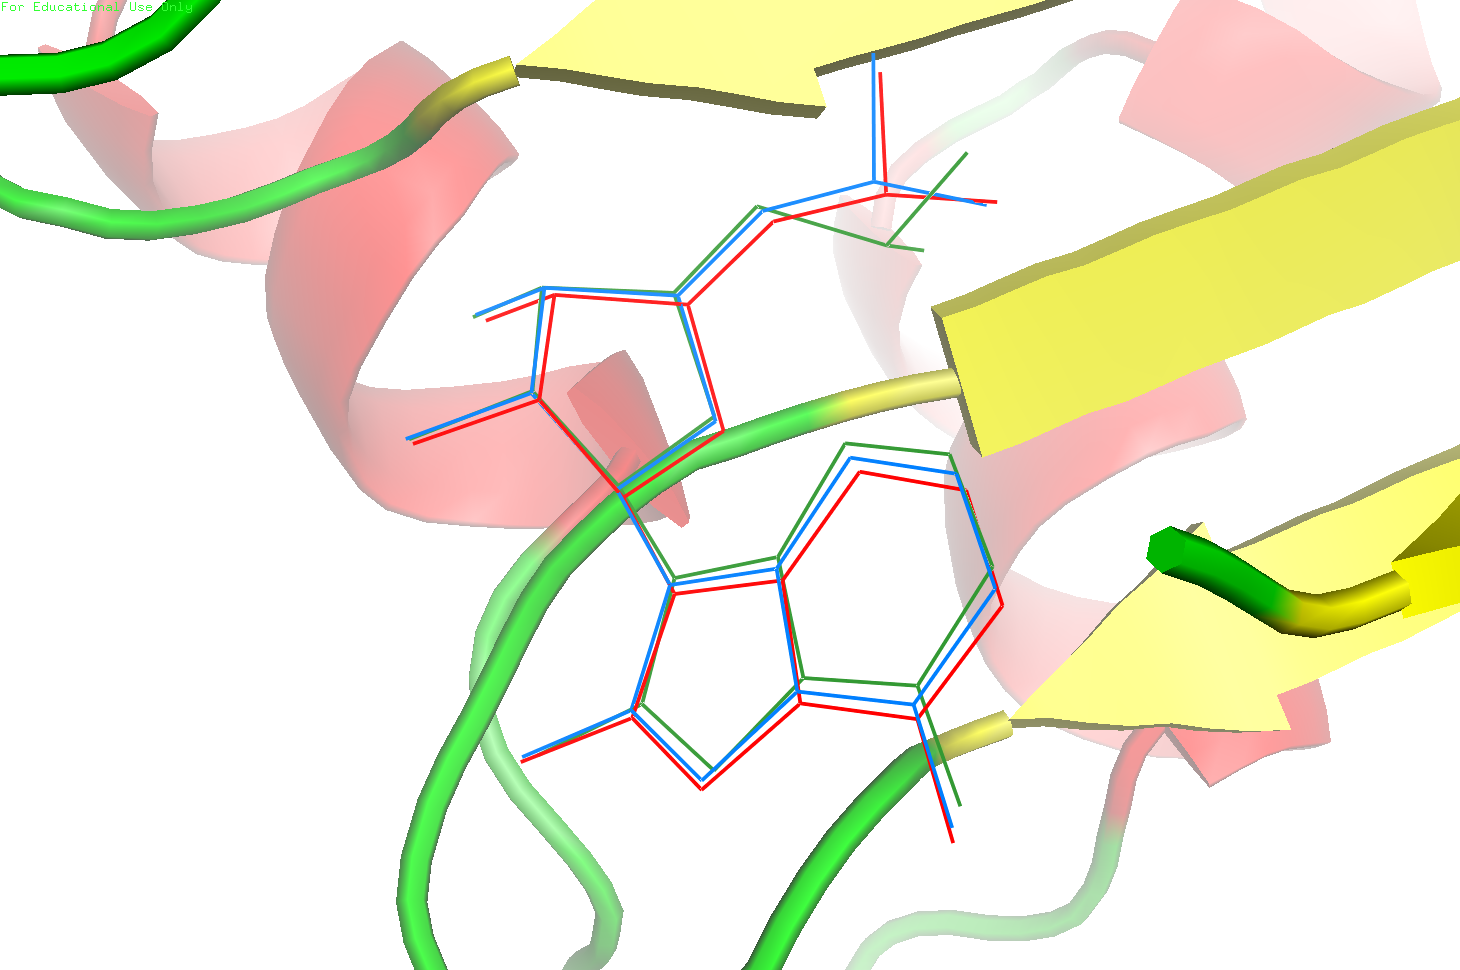
\includegraphics[width=\textwidth]{VirtualScreening/Figures/3H0W-N8M.png}
\caption{AdoMetDC in complex with crystal and docked N8M.}
\label{fig:3H0W-N8M}
\end{figure}

\begin{table}
\centering
\begin{tabular*}
{\textwidth}
{@{\extracolsep{\fill}}ccccc}
\toprule
PDB ID & Protein & Ligand & Vina (\AA) & idock (\AA) \\
\midrule
2ZD1 & HIV RT      & T27  & 0.465 & 0.555\\
1LI4  & SAHH        & NAD & 0.537 & 0.593\\
3IAR  & ADA          & 3D1 & 0.605 & 0.569\\
3BGS & PNP           & DIH & 0.756 & 1.170\\
3H0W & AdoMetDC & N8M & 0.577 & 0.600\\
\bottomrule
\end{tabular*}
\caption{RMSDs between the docked and crystal conformations of the ligands in the five protein-ligand complexes.}
\label{tab:RMSD}
\end{table}

\subsection{Virtual Screening}

Virtual screening was then carried out. 10,928 drug-like ligands were docked against the five proteins by Vina and idock. Since Vina can dock only one ligand in each run, a script containing 10,928 lines was generated and run instead, with each line being an execution of Vina to dock one individual ligand. Arguments to both programs were left as default. The GNU Time utility was used to profile both programs.

Table \ref{tab:DockingExecutionTimeComparison} compares the execution time of both programs. Vina cost 428 to 504 CPU hours for one protein. In contrast, idock cost 88 to 184T CPU hours, resulting in a speedup of 2.5 to 4.8. In terms of elapsed time, the speedup is as high as 6.3 to 10.4 because idock better utilized the computing resources.

\begin{table}[h!]
\centering
\begin{tabular*}
{\textwidth}
{@{\extracolsep{\fill}}rrrrrr}
\toprule
Program & User (s) & System (s) & CPU Hours & Elapsed & Utilization\\
\midrule
\multicolumn{6}{l}{\textbf{HIV RT}}\\
Vina	& 1656489  &	14110 &	464  & 69:15:13 &   670\%\\
idock	&   581952  &	     55 & 162  & 10:57:46 & 1474\%\\
Ratio &        2.8   & 254.3 &  2.9  &         6.3 &    0.5\\
\noalign{\smallskip\smallskip}
\multicolumn{6}{l}{\textbf{SAHH}}\\
Vina	& 1641658  &	13354 & 460 & 78:53:59 &   582\%\\
idock	&   663145  &      36 & 184 & 12:24:24 & 1484\%\\
Ratio &         2.5  &	 371.6 &  2.5 &         6.4 &   0.4\\
\noalign{\smallskip\smallskip}
\multicolumn{6}{l}{\textbf{ADA}}\\
Vina	& 1801626  &	12551 &	504 & 74:22:37 &   677\%\\
idock	&   458499  &      47 &	127 &   8:46:12 & 1452\%\\
Ratio &         3.9  &  269.7 & 4.0 &         8.5 &    0.5\\
\noalign{\smallskip\smallskip}
\multicolumn{6}{l}{\textbf{PNP}}\\
Vina	& 1526892  &	14873 & 428 & 62:19:55 &  687\%\\
idock	&   317946  &      39 &   88 &  5:58:19 & 1479\%\\
Ratio &         4.8  &  384.6 &  4.8 &       10.4 &   0.5\\
\noalign{\smallskip\smallskip}
\multicolumn{6}{l}{\textbf{AdoMetDC}}\\
Vina	& 1591186  &	14661 &	446 & 65:18:27 &   683\%\\
idock	&   517134  &	     46 &	144 &   9:49:49 & 1461\%\\
Ratio &         3.1  & 315.8 &  3.1 &         6.6 &    0.5\\
\noalign{\smallskip\smallskip}
\multicolumn{6}{l}{\textbf{Average}}\\
Vina	& 1643570  &	13910 &	460 & 70:02:02 &   660\%\\
idock	&   507735  &	     45 &	141 &   9:35:18 & 1470\%\\
Ratio &         3.2  & 311.8 &  3.3 &         7.3 &    0.4\\
\bottomrule
\end{tabular*}
\caption{Execution time comparison between AutoDock Vina and idock.}
\label{tab:DockingExecutionTimeComparison}
\end{table}

Table \ref{tab:DockingMemoryUsageComparison} compare the memory usage of both programs. idock generally consumed more memory to build grid maps at a high resolution and retained them along the way. But even so, the maximum resident set size was no more than 1.5 GB, hence idock can run on most mainstream desktop computers. Besides, idock encountered significantly fewer minor pagefaults thanks to better control of data caching and appropriate data structures.

\begin{table}[t]
\centering
\begin{tabular*}
{\textwidth}
{@{\extracolsep{\fill}}rrrr}
\toprule
Program & Max Resident (KB) & Major Pagefaults & Minor Pagefaults\\
\midrule
\multicolumn{4}{l}{\textbf{HIV RT}}\\
Vina	& 129184 & 0 & 80609435\\
idock	& 876912 & 1 &   1193579\\
\noalign{\smallskip\smallskip}
\multicolumn{4}{l}{\textbf{SAHH}}\\
Vina	&   154096 & 6 & 88088801\\
idock	& 1401040 & 1 &   1491870\\
\noalign{\smallskip\smallskip}
\multicolumn{4}{l}{\textbf{ADA}}\\
Vina	& 116384 & 0 & 71646905\\
idock	& 782752 & 0 &   1168044\\
\noalign{\smallskip\smallskip}
\multicolumn{4}{l}{\textbf{PNP}}\\
Vina	& 118416 & 0 & 71154983\\
idock	& 877344 & 1 &   1151953\\
\noalign{\smallskip\smallskip}
\multicolumn{4}{l}{\textbf{AdoMetDC}}\\
Vina	& 115312 & 0 & 70311167\\
idock	& 796272 & 1 &   1263108\\
\noalign{\smallskip\smallskip}
\multicolumn{4}{l}{\textbf{Average}}\\
Vina	& 126678 & 1.2 & 76362258\\
idock	& 946864 & 0.8 &   1253711\\
Ratio &     0.13 & 1.5 &         60.9\\
\bottomrule
\end{tabular*}
\caption{Memory usage comparison between AutoDock Vina and idock.}
\label{tab:DockingMemoryUsageComparison}
\end{table}

Table \ref{tab:DockingFreeEnergy} summarizes the statistics of predicted free energy by both programs. The free energy predicted by idock is slightly lower than the one predicted by Vina, indicating idock is slightly more likely to find the global minimum of the scoring function.

\begin{table}
\centering
\begin{tabular*}
{\textwidth}
{@{\extracolsep{\fill}}rrrrr}
\toprule
Program & Avg & Min & Max & Stdev\\
\midrule
\multicolumn{5}{l}{\textbf{HIV RT}}\\
Vina	        &	-8.7  &	-12.5 &	-2.0 & 0.9\\
idock	        &	-8.8  &	-12.8 & -2.8 & 0.9\\
Difference	&	-0.1  &	  -2.7 &  2.9 & 0.3\\
\noalign{\smallskip\smallskip}
\multicolumn{5}{l}{\textbf{SAHH}}\\
Vina	        &	-8.5  &	-12.3 & -4.7 & 1.0\\
idock       	&	-8.4  &	-12.3 & -4.7 & 1.0\\
Difference	&   0.0  &	  -2.9 & 2.5  & 0.5\\
\noalign{\smallskip\smallskip}
\multicolumn{5}{l}{\textbf{ADA}}\\
Vina	        &	-7.7  &	-10.4 &	-0.3 & 0.8\\
idock       	&	-7.7  &	-10.6 &	-2.4 & 0.8\\
Difference	&	 0.0  &	  -3.1 &   2.2 & 0.3\\
\noalign{\smallskip\smallskip}
\multicolumn{5}{l}{\textbf{PNP}}\\
Vina	        &	-7.6  &	-10.5 & -4.8 & 0.7\\
idock       	&	-7.6  &	-10.5 & -4.8 & 0.7\\
Difference	&	 0.0  &	  -1.8 &  1.7 & 0.3\\
\noalign{\smallskip\smallskip}
\multicolumn{5}{l}{\textbf{AdoMetDC}}\\
Vina	        &	-8.6  &	-12.6 &	-4.7  & 0.8\\
idock       	&	-8.6  &	-12.9 &	-4.9  & 0.8\\
Difference	&	 0.0  &	  -3.0 &   2.3  & 0.4\\
\bottomrule
\end{tabular*}
\caption{Statistics of predicted free energies in kcal/mol by AutoDock Vina and idock.}
\label{tab:DockingFreeEnergy}
\end{table}

Table \ref{tab:DockingRMSD} summarizes the statistics of RMSDs of predicted conformations by both programs. For 27\% to 40\% of all the 10,928 ligands, the RMSD of the conformations predicted by Vina and idock is equal to or less than 1.0 \AA, and for 49\% to 61\%, the RMSD is equal to or less than 2.0 \AA, indicating both programs predict similar conformations for around half of the cases.

\begin{table}
\centering
\begin{tabular*}
{\textwidth}
{@{\extracolsep{\fill}}rrrrrrr}
\toprule
Protein & $\leq$ 1.0 \AA & $\leq$ 2.0 \AA & Avg & Min & Max & Stdev\\
\midrule
HIV RT     & 40\% & 61\% & 2.554 & 0.052 & 16.409 & 2.673\\
SAHH       & 27\% & 49\% & 4.190 & 0.045 & 19.988 & 4.098\\
ADA         & 37\% & 59\% & 2.620 & 0.042 & 11.878 & 2.647\\
PNP          & 31\% & 53\% & 2.966 & 0.041 & 13.092 & 2.695\\
AdoMetDC & 38\% & 60\% & 2.643 & 0.055 & 13.032 & 2.741\\
\bottomrule
\end{tabular*}
\caption{Statistics of RMSDs of predicted conformations by AutoDock Vina and idock.}
\label{tab:DockingRMSD}
\end{table}

Filtering criteria were set in order to shortlist a few promising ligands that bind to HIV RT with high affinity but bind to the other four proteins with low affinity. Ligands whose predicted free energy against HIV RT is below -11.0 kcal/mol and whose predicted free energies against the other four proteins are above -8.5 kcal/mol were shortlisted (Table \ref{tab:ShortlistedLigands}). The ZINC19888543 predicted by Vina and the ZINC44392991 predicted by idock were further investigated. Table \ref{tab:ZINC19888543-ZINC44392991} shows their predicted xLogP, number of hydrogen bond donors (HBD), number of hydrogen bond acceptors (HBA), molecular weight (MW), and number of rotatable bonds (NRB). Figures \ref{fig:Vina-ZINC19888543} and \ref{fig:idock-ZINC44392991}, rendered by PoseView 1.0.0 \citep{748-2010}, show their binding conformations in complex with the five proteins. Hydrogen bonds, salt bridges and metal interactions are highlighted as black dashed lines. Hydrophobic interactions are highlighted as green solid lines. Pi-Pi and Pi-cation interactions are highlighted as green dashed lines. It can be seen that both ligands interact with HIV RT more intensively, particularly hydrophobic interactions and Pi-Pi interactions are more apparent.

\begin{table}
\centering
\begin{tabular*}
{\textwidth}
{@{\extracolsep{\fill}}rrrrrr}
\toprule
Ligand & HIV RT & SAHH & ADA & PNP & AdoMetDC\\
\midrule
\multicolumn{6}{l}{\textbf{Vina}}\\
ZINC04667184 & -11.1 & -6.6 & -7.5 & -7.5 & -8.0\\
ZINC06720921 & -11.0 & -7.4 & -8.0 & -8.4 & -8.5\\
ZINC14545253 & -11.0 & -6.5 & -8.0 & -7.6 & -7.9\\
ZINC19888543 & -11.1 & -7.9 & -7.8 & -7.8 & -8.4\\
ZINC26423182 & -11.1 & -6.4 & -7.8 & -7.4 & -7.3\\
ZINC49453017 & -11.3 & -7.1 & -8.3 & -7.6 & -8.4\\
ZINC60603133 & -11.0 & -7.9 & -8.3 & -7.4 & -8.5\\
\noalign{\smallskip\smallskip}
\multicolumn{6}{l}{\textbf{idock}}\\
ZINC03012460 & -11.3 & -8.3 & -7.8 & -7.3 & -8.4\\
ZINC04667184 & -11.2 & -7.6 & -7.7 & -8.0 & -8.1\\
ZINC44392991 & -11.1 & -7.7 & -7.3 & -8.1 & -7.5\\
ZINC49453017 & -11.6 & -7.3 & -8.3 & -7.8 & -8.4\\
\bottomrule
\end{tabular*}
\caption{Ligands whose predicted free energy against HIV RT is equal to or below -11.0 kcal/mol and whose predicted free energies against SAHH, ADA, PNP, and AdoMetDC are equal to or above -8.5 kcal/mol by Vina and idock.}
\label{tab:ShortlistedLigands}
\end{table}

\begin{table}
\centering
\begin{tabular*}
{\textwidth}
{@{\extracolsep{\fill}}rrrrrr}
\toprule
Ligand & xLogP & HBD & HBA & MW (Da) & NRB\\
\midrule
ZINC19888543 & 4.48 & 1 & 3 & 341.838 & 3\\
ZINC44392991 & 4.24 & 1 & 6 & 391.471 & 6\\
\bottomrule
\end{tabular*}
\caption{Chemical properties of ZINC19888543 and ZINC44392991.}
\label{tab:ZINC19888543-ZINC44392991}
\end{table}

\begin{figure}
\centering
\subfigure[HIV RT in complex with ZINC19888543.]
{
  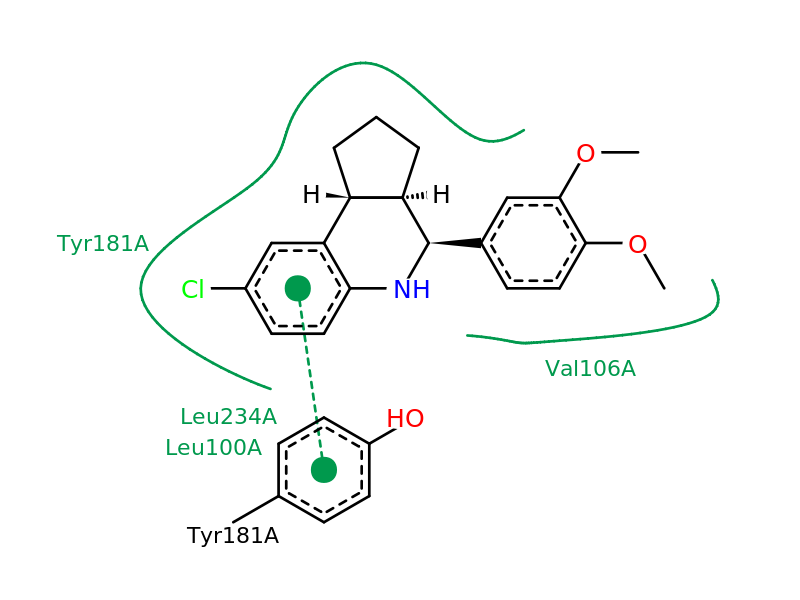
\includegraphics[width=0.47\textwidth]{VirtualScreening/Figures/2ZD1-ZINC19888543.png}
  \label{subfig:2ZD1-ZINC19888543}
}
\subfigure[SAHH in complex with ZINC19888543.]
{
  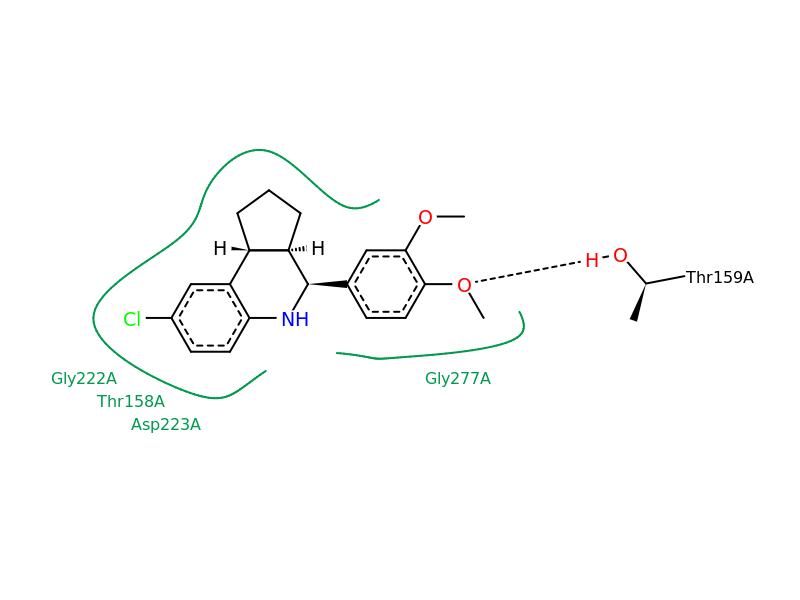
\includegraphics[width=0.47\textwidth]{VirtualScreening/Figures/1LI4-ZINC19888543.png}
  \label{subfig:1LI4-ZINC19888543}
}
\subfigure[ADA in complex with ZINC19888543.]
{
  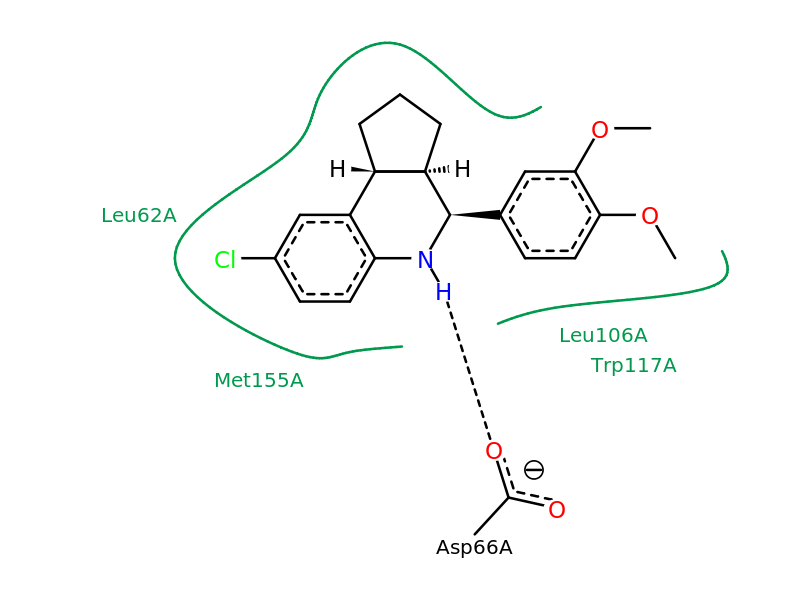
\includegraphics[width=0.47\textwidth]{VirtualScreening/Figures/3IAR-ZINC19888543.png}
  \label{subfig:3IAR-ZINC19888543}
}
\subfigure[PNP in complex with ZINC19888543.]
{
  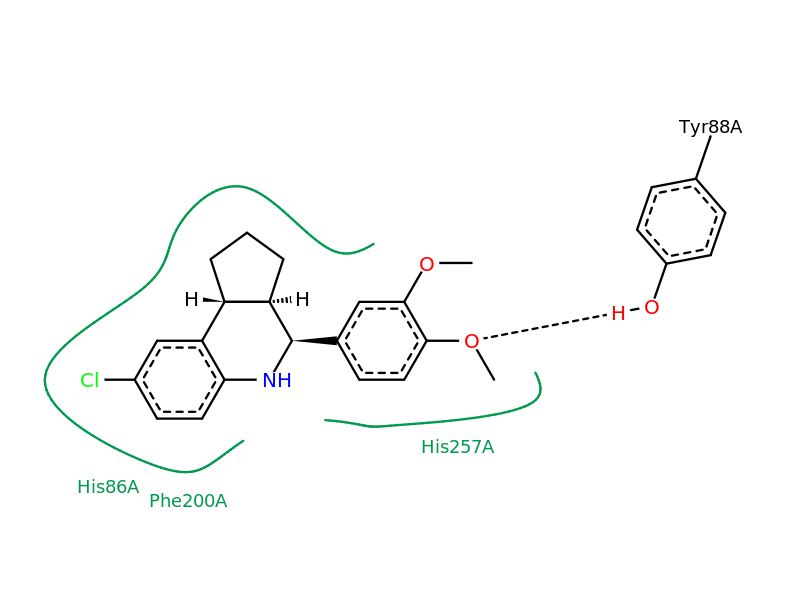
\includegraphics[width=0.47\textwidth]{VirtualScreening/Figures/3BGS-ZINC19888543.png}
  \label{subfig:3BGS-ZINC19888543}
}
\subfigure[AdoMetDC in complex with ZINC19888543.]
{
  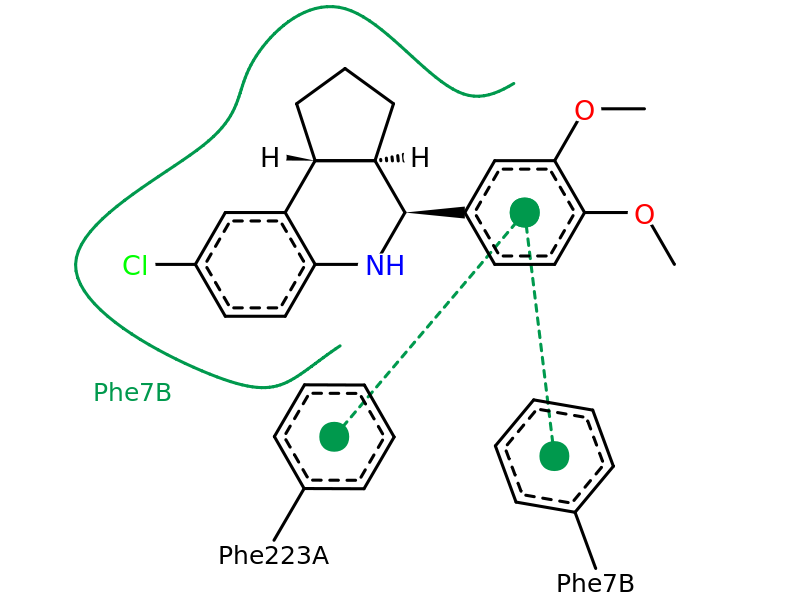
\includegraphics[width=0.47\textwidth]{VirtualScreening/Figures/3H0W-ZINC19888543.png}
  \label{subfig:3H0W-ZINC19888543}
}
\caption{HIV RT, SAHH, ADA, PNP, and AdoMetDC in complex with ZINC19888543 docked by Vina.}
\label{fig:Vina-ZINC19888543}
\end{figure}

\begin{figure}
\centering
\subfigure[HIV RT in complex with ZINC44392991.]
{
  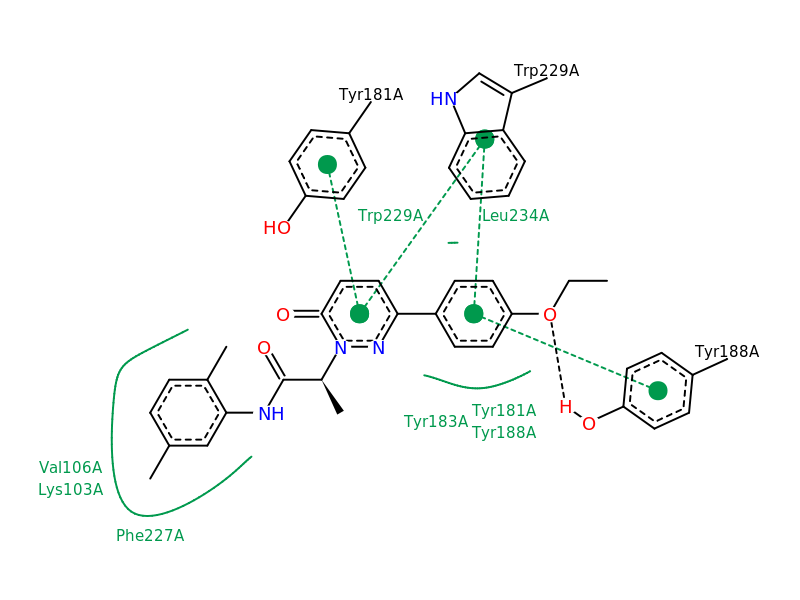
\includegraphics[width=0.47\textwidth]{VirtualScreening/Figures/2ZD1-ZINC44392991.png}
  \label{subfig:2ZD1-ZINC44392991}
}
\subfigure[SAHH in complex with ZINC44392991.]
{
  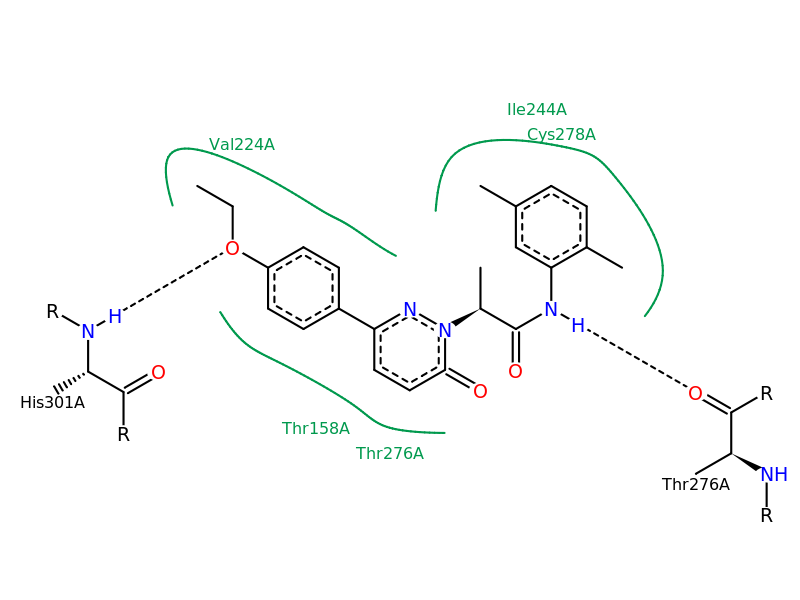
\includegraphics[width=0.47\textwidth]{VirtualScreening/Figures/1LI4-ZINC44392991.png}
  \label{subfig:1LI4-ZINC44392991}
}
\subfigure[ADA in complex with ZINC44392991.]
{
  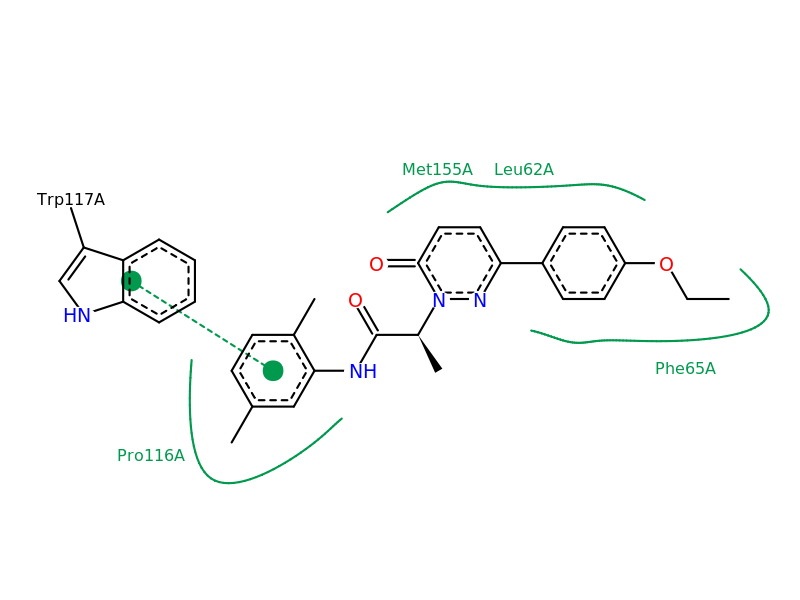
\includegraphics[width=0.47\textwidth]{VirtualScreening/Figures/3IAR-ZINC44392991.png}
  \label{subfig:3IAR-ZINC44392991}
}
\subfigure[PNP in complex with ZINC44392991.]
{
  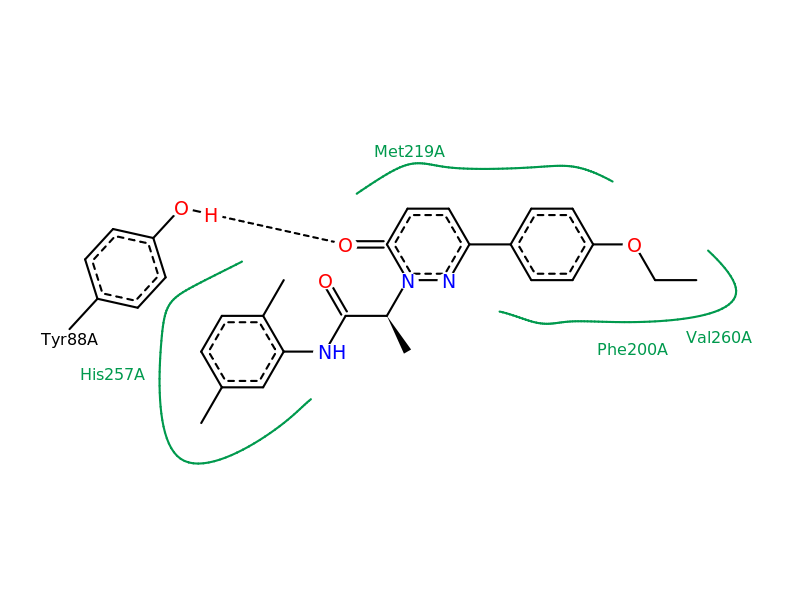
\includegraphics[width=0.47\textwidth]{VirtualScreening/Figures/3BGS-ZINC44392991.png}
  \label{subfig:3BGS-ZINC44392991}
}
\subfigure[AdoMetDC in complex with ZINC44392991.]
{
  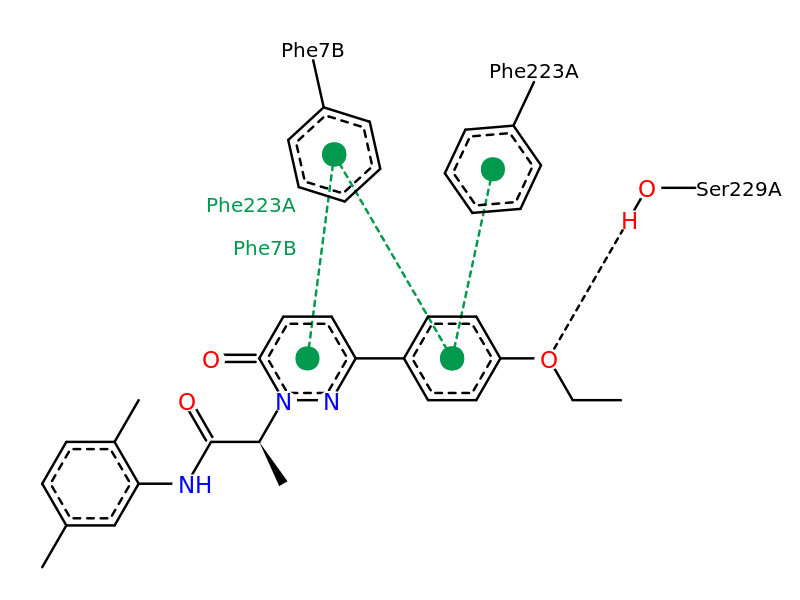
\includegraphics[width=0.47\textwidth]{VirtualScreening/Figures/3H0W-ZINC44392991.png}
  \label{subfig:3H0W-ZINC44392991}
}
\caption{HIV RT, SAHH, ADA, PNP, and AdoMetDC in complex with ZINC44392991 docked by idock.}
\label{fig:idock-ZINC44392991}
\end{figure}

\section{Discussion}

Both Vina and idock adopt the same scoring function. They differ in their C++ implementations, data structures, and Monte Carlo algorithms in finding the global minimum. idock implements its own thread pool to maintain a high CPU utilization through the entire execution. It also utilizes modern C++0x techniques such as Rvalue references to avoid frequent reallocations of array data. It abandons Vina's tree-like recursive data structures and implements flat array structures to guarantee a high data caching hit rate. It also automatically detects inactive torsions and thus reduces the dimension of variables to optimize, leading to easier findings of local minimums of the scoring function. idock has very similar input and output arguments as Vina, so it should not be hard for existing Vina users to transit to idock. However, idock does not support flexible receptor docking at the moment, so users who need this kind of docking should refer to Vina.

There are quite many requests for the support of virtual screening in Vina's forum. The birth of idock perfectly complements Vina. idock has built-in support for virtual screening. It searches for ligands in a user-specified folder and docks them one by one. It reuses the grid maps and threads across multiple ligands.

Even though idock achieved a speedup of 2.5 to 4.8 compared to Vina, it still cost around 10 hours on average to dock 10,928 ligands against a certain protein, not to mention massive dockings of millions of ligands. Virtual screening remains a time consuming practice. Faster algorithms and implementations are still highly desired. Porting idock to GPU is one of our future directions.

Having discussed with Prof. Mary Waye from School of Biomedical Sciences, we were encouraged to adopt a growing strategy to construct new ligands from an initial scaffold by adding molecular fragments heuristically, aiming to explore a larger chemical space and increase the probability of discovering novel drug candidates.

\section{Availability}

idock is hosted on CodePlex at http://idock.codeplex.com and released under Apache License 2.0. Both x86 and x64 executables for both Linux and Windows are provided. CodePlex provides discussions and issue tracking, so we will collect user feedback and update idock constantly from time to time.

\section{Conclusion}

We have developed idock, a fast tool for structure-based virtual screening. It is capable of screening 1.3 drug-like ligands per CPU minute on average, making it a competitive tool. Compared with Vina, idock achieved a speedup of 3.3x in terms of CPU time and a speedup of 7.3x in terms of elapsed time on average. It is released under an open source license, so customized improvements are encouraged.

It seems adopting a ligand growing strategy should be more appropriate for our future research. This leads to the development of our new tool for computational synthesis of potent ligands, as described in the next chapter.

\chapterend
